\setcounter{chapter}{1}

\chapter{导数与微分}

导数刻画了函数关于自变量的变化率,在现实问题中有很多对应的实例,例如:
速度、密度、压强、出生率、死亡率、曲线斜率,等等。导数的引入,极大
增强了用数学工具刻画现实问题的能力,可以说其作用是飞跃式的。

\section{导数的概念}

\subsection{函数在一点处的导数}

\begin{thx}
	函数$y=f(x)$在$x_0$的某领域内有定义,若
	$$\limdx\df{f(x_0+\dx)-f(x_0)}{\dx}$$
	存在, 则称{\bf $f(x)$在$x_0$处可导},该极限称为{\bf $f(x)$在$x_0$处的导数}, 记为
	$$f\,'(x_0),\quad \left.\df{\d y}{\d x}\right|_{x=x_0},\quad\left.\df{\d
	}{\d x}y\right|_{x=x_0},\quad \left.\df{\d }{\d x}f(x)\right|_{x=x_0}\quad
	y'_x|_{x=x_0},\quad \dot{y}(x_0)$$
\end{thx}

\begin{shaded}
	Newton把连续的量统称为{\it 流量}(fluent),把变化率称为{\it 流数}(fluxion),
	把自变量理解为时间,	时间的一个微小改变量称为{\it 瞬}(moment)。他将流量$x$的流数
	记为$\dot{x}$,二阶流数记为$\ddot{x}$,这种符号有时在{\it 动力系统}(以时间为自变量的系统)
	的讨论中还会使用,但更多的时候我们都使用现在的这套符号,它们(包括积分的符号)
	都是由Leibniz最初引入的。
\end{shaded}

在形如$\df{\d y}{\d x}$和$\df{\d}{\d x}$的导数符号中,$\df{\d}{\d x}$可以
被理解为所谓的{\it 求导算子},表示对其右方的函数求导。求导算子的优先级高于四则运算
和一般的函数运算。

{\bf 例:}假设$f\,'(x_0)$存在,则
\begin{enumerate}[(1)]
  \setlength{\itemindent}{1cm}
  \item $\limdx\df{f(x_0-\Delta x)-f(x_0)}{\Delta
  x}=$ \underline{\quad{$-f\,'(x_0)$}\quad} 
  \item $\lim\limits_{h\to 0}\df{f(x_0+2h)-f(x_0)}{h}=$
   \underline{\quad{$2f\,'(x_0)$}\quad} 
  \item $\lim\limits_{h\to 0}\df{f(x_0+h)-f(x_0-h)}{h}=$ 
  \underline{\quad{$2f\,'(x_0)$}\quad}
\end{enumerate}
以上哪个极限存在,与$f(x)$在$x_0$可导等价?

答:只有(3)与可导的定义不等价,因为其中没有提到$f(x_0)$,换言之,{\b 即便$f(x_0)$
没有定义,(3)也可能成立,但这样一来导数的定义就没有意义了!}

\subsubsection{导数的实际意义(应用背景)}

从导数的定义不难看出,导数本质上是一种{\it 变化率},严格地说,是某一点附近的
函数平均变化率的极限,在现实的问题中,有大量这种平均变化率的例子,
但有了导数,我们把这种变化率精确地与某个点(位置、时刻)对应了起来。

\begin{itemize}
  \setlength{\itemindent}{1cm}
  \item {\it 切线斜率:}
  $$k(x_0)=\lim\limits_{x\to x_0}\df{f(x)-f(x_0)}{x-x_0}$$
  \item {\it 瞬时速度:}\ps{在现实中,无法测量所谓的瞬时速度!}
  $$v(t_0)=\lim\limits_{t\to t_0}\df{S(t)-S(t_0)}{t-t_0}$$
  \item {\it 出生率:}
  $$\gamma(s_0)=\lim\limits_{s\to s_0}\df{[s_0,s]\mbox{内出生的人口总数}}{s-s_0}$$
  \item {\it 经济的增长率:}
  $$S_e=\lim\limits_{y\to y_0}\df{y\mbox{年的经济总量}
  -y_0\mbox{年的经济总量}}{y-y_0}$$
\end{itemize}

{\bf 注:}导数是函数关于自变量的变化率,也就是当自变量发生变化时,函数值发生的相应变化
与之的比率。变化率的另一种理解是{\b\it 与自变量的单位变化量对应的函数值的改变量},
例如:速度是单位时间内的位移,密度是单位体积对应的质量。

% {\bf 导数:函数关于自变量的变化率!}

{\bf 例:}已知函数$f(x)$在点$x_0$处可导,求曲线$y=f(x)$在该点的切线和法线方程。

\begin{thx}
	\begin{itemize}
% 	  \setlength{\itemindent}{1cm}
	  \item {\it 切线:\quad $y=f(x_0)+f'(x_0)(x-x_0)$}
	  \item {\it 法线:\quad $y=f(x_0)-\df1{f'(x_0)}(x-x_0)\quad(f'(x_0)\ne 0)$}
	\end{itemize}
\end{thx}
{\bf 例:}若抛物线$y=x^2$上有三个不同号点处的法线交于一点,这三个点的横坐标需要满足什么条件?

[提示]: 设三个点的横坐标分别是$a_1,a_2,a_3$。

情形一:若某个$a_i=0$(不妨为$a_1=0$),显然由对称性可知,必有$a_2=-a_3$。

情形二:若$a_1,a_2,a_3$均非零,我们可以给出$a_i(i=1,2,3)$处的法线方程
$$y=a_i^2-\df1{2a_i}(x-a_i)$$
化简后可得
$$\df{a_1+a_2}{a_3}=\df{a_1+a_3}{a_2}=\df{a_2+a_3}{a_1}$$
进而
$$\df{a_1+a_2+a_3}{a_3}=\df{a_1+a_2+a_3}{a_2}=\df{a_1+a_2+a_3}{a_1}$$
显然$a_,a_2,a_3$相互不同,故必有$a_1+a_2+a_3=0$。

{\bf 思考:}可导等价于存在切线吗?

[答]:否,可导则必存在切线,反之不然。若切线是铅直方向的,则导数没有意义!
例如:函数$f(x)=\sqrt[3]x$在点$x=0$不可导(导数为$\infty$),
但存在切线(铅直方向)。

\subsubsection{导数存在的条件}

为了讨论的方便,我们有时会使用“{\it 左(右)导数}”的概念,对应于导数定义中分别取
左(右)导数的情形,记为{\b$f'_-(x_0)$}和{\b$f'_+(x_0)$},
显然由导数的定义,$f(x)$在$x_0$可导,当且仅当在该点的左、右导数存在且相等。


% {\bf 定理:}初等函数在其定义域内是处处可导的。\ps{而且其任意阶导函数也是可导的!}
% 
% 这个定理我们

不难证明,函数在一点连续是在该点可导的一个必要条件。

\begin{thx}
	{\bf 定理:}$f(x)$在一点可导,则一定在该点连续。
\end{thx}

[证]:设$f(x)$在$x_0$可导,导数为$A$,则
\begin{align*}
	\limx{x_0}[f(x)-f(x_0)]
	&=\limx{x_0}\df{f(x)-f(x_0)}{x-x_0}\cdot(x-x_0)\\
	&=\limx{x_0}\df{f(x)-f(x_0)}{x-x_0}\limx{x_0}(x-x_0)\\
	&=A\cdot 0=0,
\end{align*}
从而可知$\limx{x_0}f(x)=f(x_0)$,也即$f(x)$在$x_0$连续。
\hfill$\Box$

{\bf 例:}已知$f(x)$在$x=0$连续,且$\limx{0}\df{f(x)}x=A$,
证明$f(x)$在$x=0$可导,并求$f'(0)$。

[解]:由$f(x)$在$x=0$连续,
$$f(0)=\limx0f(x)=\limx0\df{f(x)}x\cdot x
=\limx0\df{f(x)}x\cdot\limx0x=A\cdot 0=0,$$
从而
$$A=\limx{0}\df{f(x)}x=\limx{0}\df{f(x)-f(0)}{x-0}=f'(0),$$
由此可知$f(x)$在$x=0$可导,且$f'(0)=A$。
\hfill$\Box$

当然,连续并不是可导的充分条件,例如$f(x)=|x|$在$x_0$处连续,但不可导,
其左右导数分别为$\pm 1$。

{\bf 讨论:}函数在一点不可导,可能有哪些不同的形态?

[提示]:不连续、切线为铅直方向或尖点,如图

\begin{center}
	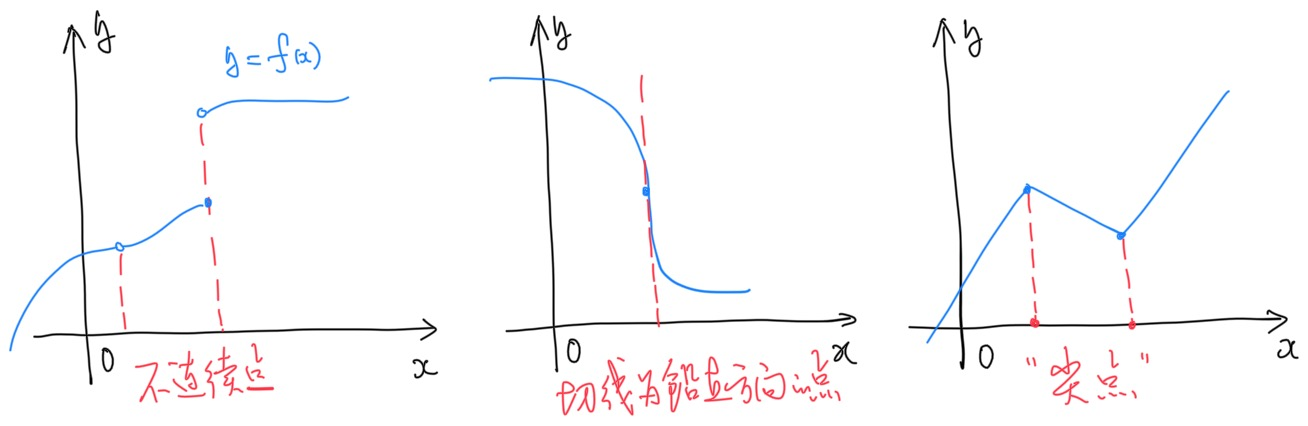
\includegraphics[width=0.9\textwidth]{./images/ch2/nDeri.jpg}
\end{center}

{\bf 例:}函数$f(x)=x^2D(x)$在$x=0$可导,但在其他地方都不连续。

[证]:注意到$0\leq x^2D(x)\leq x^2$,故对任意$x\ne 0$,
$$0\leq \df{x^2D(x)}{x}\leq x,$$
从而由夹逼定理,可知
$$\limx{0}\df{f(x)-f(0)}{x-0}=\limx{0}\df{x^2D(x)}{x}=0,$$
即证。
\hfill$\Box$

\begin{shaded}
	连续但不可导最极端的情况是如下的{\kaishu Weierstrass函数},
	可以证明(涉及函数项级数的一些性质,在此不作证明)它在处处连续但处处不可导:	
	$$W(x)=\sum\limits_{n=0}^{\infty}a^n\cos(b^n\pi x),$$
	其中$a\in(0,1)$,$b$为正的奇数,满足$ab>1+\df32\pi$
	\begin{center}
		\resizebox{!}{6cm}{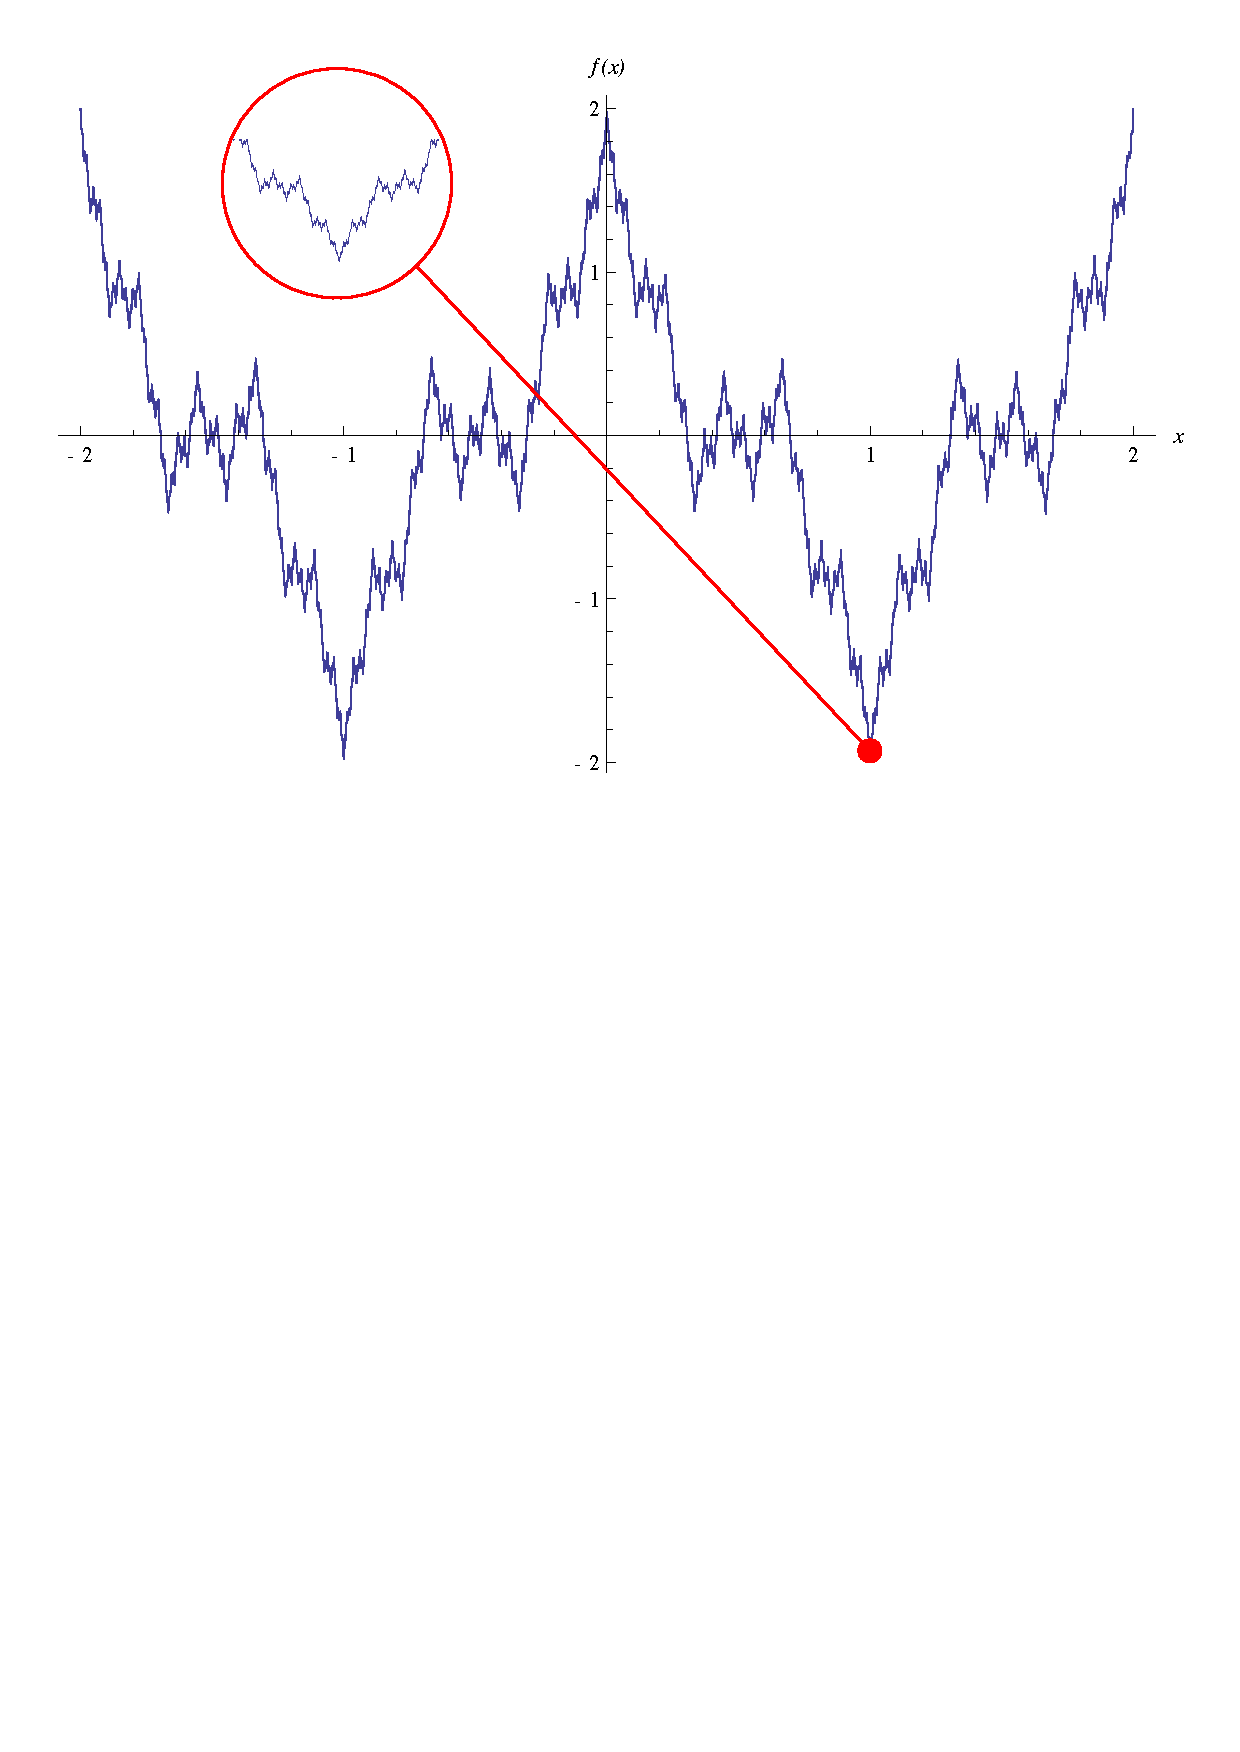
\includegraphics{./images/ch4/WFunc.pdf}}
		
		\kaishu Weierstrass函数具有某种“分形”的特征,对其任何一个微小的局部
		进行放大,都会呈现处相似的锯齿状形态,它是一个真正在任一段上都不光滑的函数。
	\end{center}
	
	这个反例的引入对数学界造成了巨大的震动,但同时也产生了无可替代的巨大意义。
	《微积分的历程》一书中(P.169)的一段评述可以给我们启发:{\it 在持续不断的起伏中,数学家们建立起
	雄伟的理论体系,然后寻找足以揭示他们的思想界限的恰当反例。这种理论与反例的对照
	成为正确推理的引擎,凭借这种工具,数学得以进步。因为{\b 我们唯有知道某些特性是如何
	丧失的,方能了解它们是怎样发挥作用的。同样,我们唯有认清直觉是如何把人引入歧途
	的,方能如实地评价推理的威力。}}
\end{shaded}

{\bf 例:}确定常数$a,b$的值,使得函数
$$f(x)=\left\{\begin{array}{ll}ax+b,& x>0\\
e^x,& x\leq 0\end{array}\right.$$
在$x=0$可导。

{\bf 注:}{\b 计算分段定义的函数的导数,在分段的点上的左右导数要分别计算,
其他(可导区间上的)部分直接利用常用的求导公式即可!}

{\bf 例:}问题讨论
\begin{enumerate}[(1)]
  \setlength{\itemindent}{1cm}
  \item 若$f(x),g(x)$在$x_0$均不可导,是否$f(x)+g(x),$ $f(x)g(x)$必不可导?
  ({$\times$}) 
  
  [反例]:$f(x)=D(x)$,$g(x)=1-D(x)$。
  \item 若对任意$x\in (a,b)$,恒有$f(x)<g(x)$,且$f(x),g(x)$均在$(a,b)$内
  可导,问是否必有$f\,'(x)<g'(x)$? ({$\times$})
  
  [反例]:$f(x)=\sin x$,$g(x)=2$。 
  \item $f(x)$可导,则$|f(x)|$可导?反之呢?({$\times$})
  
  [反例]:都错误,$f(x)=x$,$|f(x)|=|x|$在$x=0$不可导;反之,考虑$f(x)=D(x)-\df12$。
  \item 若$f(x)$在$\mathbb{R}$上可导,且$\limx{+\infty}f(x)=\infty$,是否
  必有$\limx{+\infty}f\,'(x)=\infty$?反之呢? ({$\times$})
  
  [反例]:$f(x)=x$。
  \item 若$f(x)$在$(a,b)$内可导,且$\limx{a^+}f(x)=\infty$,是否
  必有$\limx{a^+}f\,'(x)=\infty$? 反之呢?({$\times$})
  
  [反例]:$f(x)=\df1x+\sin\df1x$。 
  \item {\b 若$f(x)$可导且为奇(偶)函数,则$f\,'(x)$也有奇偶性? 
  (相应的$f'(0)$有什么特点?偶函数,$f'(0)=0$)({$\surd$})} 
  \item {\b 若$f(x)$可导且为周期函数,则$f\,'(x)$也是周期函数? ({$\surd$})}
\end{enumerate}

% {\bf 例:}设$f(x)=\sum\limits_{i=1}^na_i\sin
% ix$,其中$a_i(i=1,2,\ldots,n)$为常数,且对任意$x\in\mathbb{R}$, 
% $|f(x)|\leq |\sin x|$,证明:
% $$\left|a_1+2a_2+\ldots+na_n\right|\leq 1$$
% 
% [提示]:$f(0)=0$,于是
% $$|f'(0)|=\limx{0}\df{|f(x)|}{|x|}\leq\limx{0}\df{|\sin x|}{|x|}=1$$
% 事实上$f'(0)=a_1+2a_2+\ldots+na_n$.

{\bf 思考:}
\begin{enumerate} 
  \setlength{\itemindent}{1cm}
  \item {\b $f'(x_0)$和$[f(x_0)]'$,$f'(x)$和$[f(x)]'$有何异同?}
  \item {\b $f'_+(x_0)$和$f'(x_0+0)$有何区别?}
  \ps{有些书上也把$f'(x_0+0)$记为$f'(x_0^+)$}
  \item $f(x)=g(x)$可推出$f'(x)=g'(x)$?反之呢?
  \item 圆的面积$S(r)$关于直径的导数$S'(r)=l(r)$为圆周长,
  球体积关于直径的导数为表面积,如何解释?类似的,(定长)圆柱体的体积关于截面半径的导数
  等于其与侧面积?矩形的体积关于各边长的导数等于其对应的截面积?
\end{enumerate}

\subsection{导函数}

有了函数在一点的导数概念,可以很容易地将其扩展到所谓的{\it 导函数},也即由函数
在不同点处的导数值所构成的函数。为了今后的讨论方便,不加证明地引入如下定理:

\begin{thx}
	{\bf 初等函数的可导性:}所有初等函数在其定义域内均是处处可导的。
\end{thx}

事实上,经过本章稍后的讨论,我们会发现,初等函数的导函数都是初等函数。
但是,需要提醒一句的是,并非只有初等函数的导函数才是初等函数。例如没有一个
初等函数的导函数是$e^{x^2}$或者$\df{\sin x}x$。

接下来我们的主要任务就是给出所有初等函数的导函数。

利用导数的定义和基本的极限运算,可以很容易地求出一些常用初等函数的导函数:

\begin{thx}
	{\bf 一些常用函数的导函数}
	\begin{enumerate}[(1)]
% 	  \setlength{\itemindent}{1cm}
	  \item $f(x)=C\;(C\mbox{为常数})$ \hfill $f\,'(x)=0$ 
	  \item $f(x)=x^n\;(n\in\mathbb{Z})$ \hfill $f\,'(x)=nx^{n-1}\,(n\ne
	  0)$ 
	  \item $f(x)=e^x$ \hfill $f\,'(x)=e^x$ 
	  \item $f(x)={\color{red}\ln|x|}$ \hfill $f\,'(x)=\df 1x$ 
	  \item $f(x)=\sin x$ \hfill $f\,'(x)=\cos x=\sin\left(x+\df{\pi}2\right)$ 
	  \item $f(x)=\cos x$ \hfill $f\,'(x)=-\sin x=\cos\left(x+\df{\pi}2\right)$
	\end{enumerate}
\end{thx}

\begin{ext}
	{\centering\bf 课后作业}
	
	\begin{enumerate}  
% 	  \item 确定$a$的值,使$y=ax^2$与$y=\ln x$相切。
	  \item 已知$f(x)=\left\{\begin{array}{ll}
		2e^x+b,& x\leq0\\ ax+\sin x,& x> 0
		\end{array}\right.$
		试确定$a,b$的值,使得$f(x)$在$x=0$处可导。
% 	  \item 求曲线$y=\cos x$在$\left(\df{\pi}3,\df12\right)$处的切线和
% 	  法线方程。
	  \item 证明:曲线$xy=a^2$上任一点处的切线与两坐标轴构成的三角形面积不变。
	  \item 讨论函数
	  	$y=\left\{\begin{array}{ll}
	    	x^2\sin\df1x,& x\ne0;\\ 0, & x=0.
	    \end{array}\right.$
	  在$x=0$处的连续性、可导性以及导函数的连续性。
	  \item 设对任意$x\in\mathbb{R}$,均有$f(x+2)=f(x)$,已知$f'(0)=1$,
	  证明$f(x)$在$x=2$可导,并求$f'(2)$。
	  \item 已知曲线$y=f(x)$和曲线$y=\sin x$在原点相切(即二者的切线相同),
	  求$\limx0\df{f(3x)}x$。
% 	  \begin{enumerate}[(1)]
% 	    \item 
% 	    \item $y=\left\{\begin{array}{ll}
% 	    	x^2\sin\df1x,& x\ne0;\\ 0, & x=0.
% 	    \end{array}\right.$
% 	  \end{enumerate}
	  \item (选作)已知$f'(a)f(a)\ne 0$,求
	  $\limx0\left[\df{f(a+x)}{f(a)}\right]^{\frac1{\sin x}}.$
	  \item (选作)设对任意$x,y\in\mathbb{R}$,有
	  $$f(x+y)=f(x)+f(y)+x^2y+xy^2,$$
	  且当$x\to0$时$f(x)$与$x$是等价无穷小,证明$f(x)$处处可导,并求其导函数。
	\end{enumerate}
\end{ext}

\section{函数的求导法则}

\subsection{四则运算的求导法则}

\begin{thx}
	{\bf 四则运算求导公式:}设$u(x),v(x)$均在$x$可导,则
	\begin{enumerate}[(1)]
% 	  \setlength{\itemindent}{1cm}
	  \item $[u(x)\pm v(x)]'=u'(x)\pm v'(x)$ 
	  \item $[u(x)v(x)]' =u'(x)v(x)+u(x)v'(x)$ 
	  \item $\left[\df{u(x)}{v(x)}\right]'
	  =\df{u'(x)v(x)-u(x)v'(x)}{v^2(x)}\;\;(\mbox{假设}v(x)\ne 0)$
	\end{enumerate}
\end{thx}

{\bf 思考:}自行推导$(uvw)'$的公式,并给出类似函数的求导规律。

{\bf 例:}计算以下函数的导函数
\begin{enumerate}[(1)]
  \setlength{\itemindent}{1cm}
  \item $f(x)=2x^3+3x-4x+5-\df 6x$ 
  \item $f(x)=e^x\sin x$ 
  \item $f(x)=\df{x-1}{x+1}$ 
  \item $f(x)=\df 1{\ln x}$ 
  \item \tcbox[tcbox raise base,colframe=blue!40!black,colback=white]
  {$f(x)=\tan x$ \hspace{8cm}  $f\,'(x)=\sec^2 x$}
  \item \tcbox[tcbox raise base,colframe=blue!40!black,colback=white]
  {$f(x)=\sec x$ \hspace{7.5cm} $f\,'(x)=\sec x\tan x$}
\end{enumerate}

{\bf 例:}已知$f(x)$可导,且无零点,证明:$y=f(x)$和$y=f(x)\sin x$
在相交的位置必相切。

\begin{shaded}
	{\bf 关于$f(x)\sin x$的图像}
	
	在本门课程中,形如$f(x)\sin x$的函数常常用来作为讨论的示例,为此,了解一下
	有关函数的大致形态是很有必要的。请自行分析一下这些函数的图像有什么共性和差异。
	\begin{center}
		\resizebox{!}{4cm}{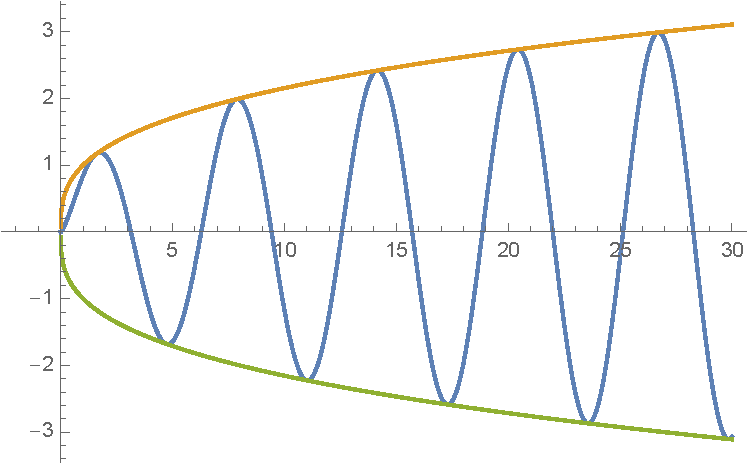
\includegraphics{./images/ch4/x3Sinx.pdf}}\quad
		\resizebox{!}{4cm}{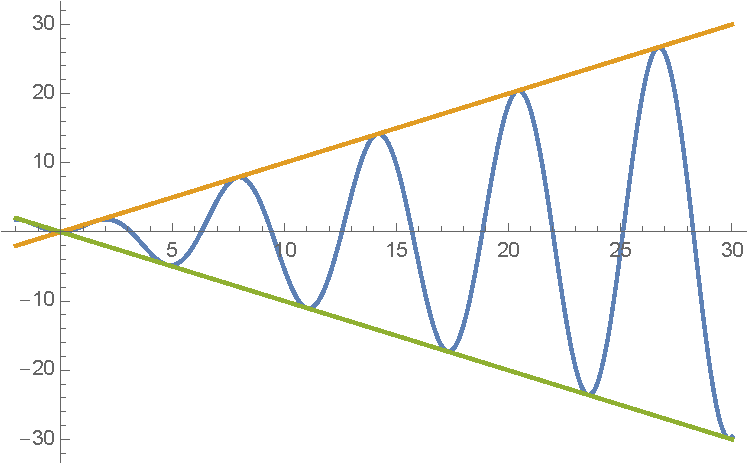
\includegraphics{./images/ch4/xSinx.pdf}}
		
		$y=x^{1/3}\sin x$\hspace{5cm}$y=x\sin x$
		
		\resizebox{!}{4cm}{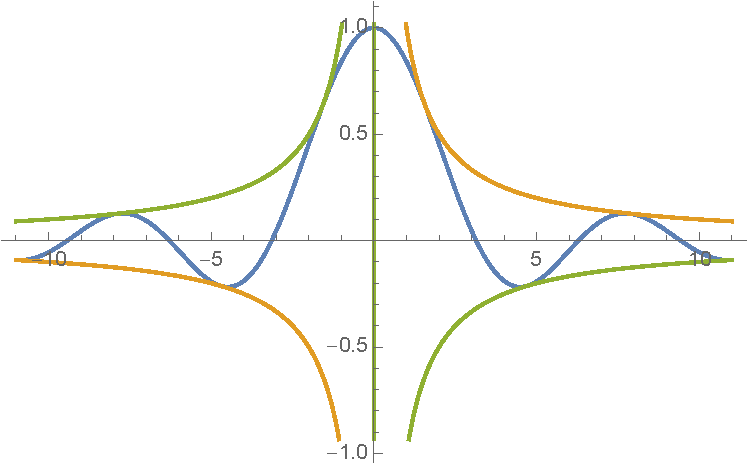
\includegraphics{./images/ch4/1xSinx.pdf}}\quad
		\resizebox{!}{4cm}{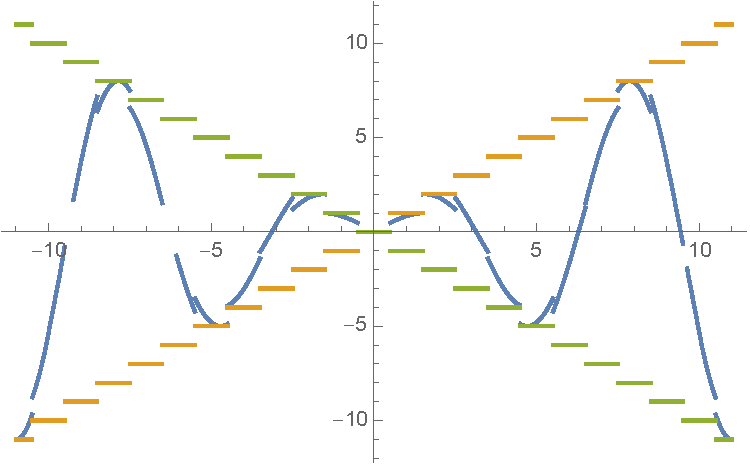
\includegraphics{./images/ch4/rxSinx.pdf}}
		
		$y=\df1x\sin x$\hspace{5cm}$y=[x]\sin x$
		
		\resizebox{!}{4cm}{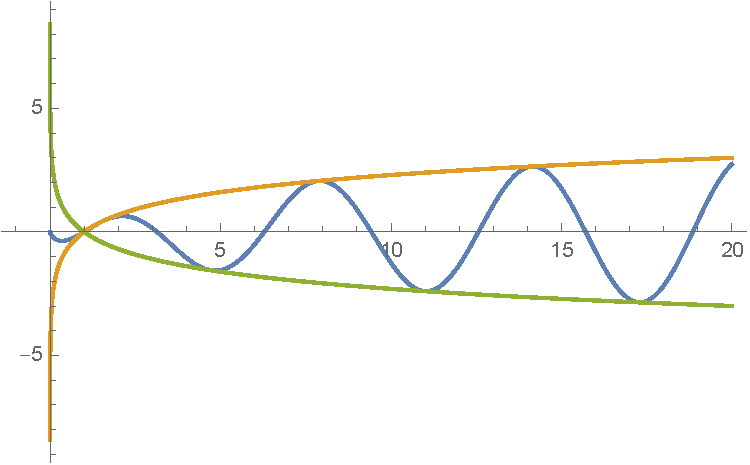
\includegraphics{./images/ch4/lnxSinx.pdf}}\quad
		\resizebox{!}{4cm}{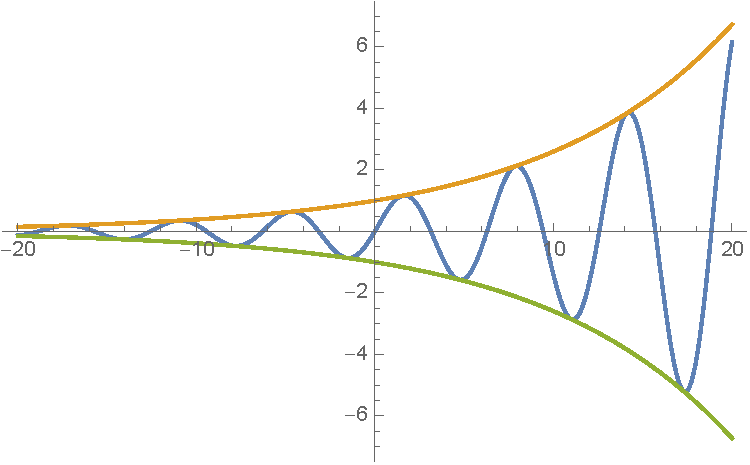
\includegraphics{./images/ch4/11xSinx.pdf}}
		
		$y=\ln x\sin x$\hspace{5cm}$y=1.1^x\sin x$
		
		\kaishu $y=f(x)$和$y=f(x)\sin x$的图像在相交的位置必相切
	\end{center}
\end{shaded}

\subsection{反函数求导法则}

自变量和因变量(函数)是一种相对的关系,将原来的因变量视为自变量,通过反函数来研究
原来的自变量的变化规律,是一种常见的数学手段。为此,讨论反函数的变化率(导数)就显得非常
有必要了。

假设函数$y=f(x)$可逆,其反函数为$x=g(y)$。设$\Delta x$和$\Delta y$
为自变量和因变量在$x$处对应的变化量。若$f(x)$可导,则必连续,从而
$$\lim\limits_{\Delta x\to 0}\Delta y=0,$$
又$f(x)$可逆,故必为一一映射,从而可知$\Delta x\to0\Leftrightarrow\Delta y\to0$。
于是由
$$f'(x)=\lim\limits_{\Delta x\to 0}\df{\Delta y}{\Delta x},$$
如果$f'(x)\ne 0$,则上式两边求倒数可得
$$
	\df1{f'(x)}=\lim\limits_{\Delta x\to 0}\df{\Delta x}{\Delta y}
	=\lim\limits_{\Delta y\to 0}\df{\Delta x}{\Delta y}
$$
再由导数的定义,上式右端就是$g'(y)$。

至此,我们可以得到如下的结论:

\begin{thx}
	{\bf 反函数求导公式:}设$y=f(x)$和$x=g(y)$互为反函数,若$f(x)$可导,且$f'(x)\ne 0$,则
	$$g'(y)=\df1{f'(x)}.$$
\end{thx}
注意,{\b 使用反函数的求导公式时,必须注意原函数和反函数的自变量是不同的,
因此求导的时候$f'(x)$和$g'(y)$实际上分别是$f'_x(x)$和$g'_y(y)$。}

{\bf 例:}考虑函数$y=e^x$,我们已知$(e^x)'_{\b x}=e^x$,故
\begin{thx}
	$$(\ln y)'_{\b y}=\df1{(e^x)'_{\b x}}=\df1{e^x}=\df1y$$
\end{thx}

{\bf 例:}计算下列函数的导函数
\begin{enumerate}[(1)]
  \setlength{\itemindent}{1cm}
  \item \tcbox[tcbox raise base,colframe=blue!40!black,colback=white]
  {$f(x)=\arcsin x$ \hspace{6.9cm} $f\,'(x)=\df{1}{\sqrt{1-x^2}}$} 
  \item \tcbox[tcbox raise base,colframe=blue!40!black,colback=white]
  {$f(x)=\arctan x$ \hspace{7.2cm} $f\,'(x)=\df{1}{1+x^2}$}
\end{enumerate}

[提示]:记$y=\sin x$,则
$$(\arcsin x)'_{\b x}=\df1{(\sin y)'_{\b y}}=\df1{\cos y}
=\df1{\sqrt{1-\sin y}}=\df1{\sqrt{1-x^2}}.$$

{\bf 例:}设$f(x)=x^5+2x^3+4x,(-\infty<x<+\infty)$
\begin{enumerate}[(1)]
  \setlength{\itemindent}{1cm}
  \item 证明$f$可逆;
  \item 设$g=f^{-1}$,计算$g(7)$
  \item 计算$g'(7)$
\end{enumerate}

\subsection{复合函数的求导法则}

利用函数的复合运算来构造新的函数,或者说将一些函数看成是常见函数的复合,
也是常见的一种情况,这时我们常常需要讨论复合函数的极限。

假设$u=f(x),y=g(u)$均可导,于是若将$y$视为$x$的复合函数,设
$\Delta x,\Delta u,\Delta y$为相对应的三个变化量,则有
\begin{align*}
	\lim\limits_{\Delta x\to 0}\df{\Delta y}{\Delta x}
	&=\lim\limits_{\Delta x\to 0}\df{\Delta y}{\Delta u}
	\cdot\df{\Delta u}{\Delta x}
	=\lim\limits_{\Delta x\to 0}\df{\Delta y}{\Delta u}
	\cdot\lim\limits_{\Delta x\to 0}\df{\Delta u}{\Delta x}\\
	&=\lim\limits_{\Delta u\to 0}\df{\Delta y}{\Delta u}
	\cdot\lim\limits_{\Delta x\to 0}\df{\Delta u}{\Delta x}
	=g'(u)f'(x)=g'(f(x))f'(x),
\end{align*}
于是,我们得到了如下的关于复合函数的求导法则
\begin{thx}
	$$[g(f(x))]'=g'(f(x))\cdot f'(x).$$
\end{thx}
试想一下,如果是三个可导的函数相互复合,则由
$$[h(g(f(x))]'=h'(g(f(x)))\cdot g'(f(x))\cdot f'(x),$$
这很类似于一环一环地解开一个相互连接的链条,因此该法则也被称为{\it 链式法则}。


{\bf 例:}幂函数和指数函数的导函数
\begin{thx}
	\begin{enumerate}[(1)]
	%   \setlength{\itemindent}{1cm}
	  \item $y=a^x\;(a>0,a\ne 1)$ \hfill $y'=a^x\ln a$ 
	  \item $y=x^a$ \hfill $y'=ax^{a-1}$
	\end{enumerate}
\end{thx}

[提示]:
$$(a^x)'=[e^{x\ln a}]'=e^{x\ln a}\cdot (x\ln a)'=a^x\ln a.$$

请注意,到目前为止,我们终于得到了所有基本初等函数的求导公式。接下来,我们可以利用
这些基本的公式,结合求导法则,来求各种函数的导函数了。

{\bf 例:}若$f$可导,且$[f(x^2)]'=[f^2(x)]'$,则$f(1)=1$或$f'(1)=0$.

[提示]:
$$[f(x^2)]'=f'(x^2)\cdot (x^2)'=2xf'(x),
\quad [f^2(x)]'=2f(x)\cdot f'(x).$$
令$x=1$,代入比较即得。

{\bf 例:}计算下列函数的导函数
\begin{enumerate}[(1)]
  \setlength{\itemindent}{1cm}
  \item $y=e^{x^2}$ 
  \item $y=\sin (3x+2)$ 
  \item $y=\cos^2(1-2x)$ 
  \item $y=\ln\sin e^{-x}$ 
  \item $y=(1-30x)^{50}$ 
  \item $y=\ln(1+x^2)$ 
  \item $y=e^{\sqrt{1-3x}}$ 
  \item $y=x^x$ 
  \item $y=e^{\tan\frac 1x}$
\end{enumerate}

{\bf 例:}形如$y=u^v$的函数求导,其中$u,v$均可导
\begin{enumerate}[(1)]
  \setlength{\itemindent}{1cm}
  \item $y=x^x$
  
  [提示]:
  $${\b (x^x)'=(e^{x\ln x})'=e^{x\ln x}\left(\ln x+x\cdot\df1x\right)
  =x^x(1+\ln x)}$$
  \item $y=x^{x^x}$
  \item $y=\left(x^x\right)^x$
\end{enumerate}

计算此类题目,必须注意的一点形如$u^v$的函数并不属于任何一类基本初等函数,因此必须首先将其
转换为基本初等函数的复合函数形式,再用复合函数的求导法则来求导。

对于这类题目,另一个常见的求导方法是所谓的“{\it 对数求导法}”,
先对函数取对数,然后再求导,例如:
$$\ln(u^v)=v\ln u,$$
两边分别求导
$$[\ln(u^v)]=\df{(u^v)'}{u^v},
\quad (v\ln u)'=\ln u+\df vu,$$
故
$$(u^v)'=u^v\left(\ln u+\df vu\right).$$
对于多个函数相乘构成的函数求导,采用先取对数再求导的方式也是非常高效的。

{\bf 例:}求下列函数的导函数
\begin{enumerate}[(1)]
  \setlength{\itemindent}{1cm}
  \item $y=x\sqrt{\df{1-x}{1+x}}$,
  \item $y=\df{x^2}{1-x}\sqrt[3]{\df{3-x}{(3+x)^2}}$. 
\end{enumerate}

\begin{ext}
	{\centering\bf 课后作业}
	
	\begin{enumerate}  
	  \item 同济教材-习题2-2:7,8;
	  \item 计算如下函数的导函数
	  \begin{enumerate}[(1)]
	    \item $y=\arcsin\sqrt{1-x^2}$,
	    \item $y=\ln(e^x+\sqrt{1+e^2x})$,
	    \item $y=\arctan\sqrt{x^2-1}-\df{\ln x}{\sqrt{x^2-1}}$,
	    \item $y=\ln\tan\df x2-\cos x\ln\tan x$,
	    \item $y=\left(1+\df1x\right)^x$,
	    \item $y=x^2+2^x+x^x+2^2$,
	    \item $y=\sqrt{x+\sqrt{x+\sqrt x}}$.
	  \end{enumerate}
	  \item 已知函数$g(x)$在$x=a$连续,问函数$f(x)=|(x-a)|g(x)$
	  在$x=a$是否可导?若可导,证明之;若不可导,讨论增加什么样的条件可以使之可导。
	  利用以上讨论的结果,判断$f(x)=(x^2-4)|x^2+3x+2|$有几个不可导的点。
	  \item 设$f(x)$可导,且$f\,'\left(\df{\pi}{4}\right)=1$,求
		$$\left.f'\left(\arctan\df{1+x}{1-x}\right)\right|_{x=0}
		\quad\mbox{和}\quad  
		\left[f\left(\arctan\df{1+x}{1-x}\right)\right]'_{x=0}.$$
% 		在$x=0$处的导数。
% 	  \item 求$\left(1+\df1x\right)^x$和$x\sqrt{\sin x\sqrt{1-e^x}}$的导函数。
	  \item 自行完成不少于100道各种求导计算题({\it\b 不用写在作业本上})。 
	\end{enumerate}
\end{ext}

\section{高阶导数}

高阶导数就是导函数的导数,并且可以依次递推,
\begin{thx}
	{\bf $f(x)$的$n$阶导数}:
	$$f^{\,(n)}(x)=\df{\d^nf(x)}{\d x^n}
	=\df{\d}{\d x}f^{(n-1)}(x)
	=\left[f^{\,(n-1)}(x)\right]'_x$$
	
\end{thx}

{\bf 例:}求函数$f(x)=x^3+2x^2-3x+10$的各阶导函数。

多项式函数在可导性方面具有非常“优良”的性质:任意阶可导,且若求导阶数高于其次数
(最高次幂的幂次),则对应的高阶导数恒为零。也即,{\b 若$P(x)$为$n$次多项式,
则$P^{(n+1)}(x)\equiv0$}。

对于一般的函数,如果要求出其各阶导函数,则需要通过观察寻找规律,而大多数函数的高阶导数
是很难找到通用的表示的。下面一些高阶导数有比较明显规律的例子:

{\bf 例:}求以下函数的$n$阶导数
\begin{enumerate}[(1)]
  \setlength{\itemindent}{1cm}
  \item $y=\df 1x$ \hfill $y^{(n)}(x)=(-1)^n\df{n!}{x^{n+1}}$ 
  \item {\b$y=\sin x$ \hfill
  $y^{(n)}(x)=\sin\left(\df{n\pi}{2}+x\right)$} 
  \item {\b$y=xe^x$ \hfill $y^{(n)}(x)=(n+x)e^x$}
  \item $y=e^{ax}\sin bx$

[提示]:(4)
$$y'=e^{ax}(a\sin bx+b\cos
bx)=\sqrt{a^2+b^2}e^{ax}\sin(bx+\varphi),
\;\tan\varphi=\df ba$$
$$y^{(n)}=\left(a^2+b^2\right)^{n/2}e^{ax}\sin(bx+n\varphi)$$ 
\end{enumerate}

\subsection{Leibniz公式}

对于形如$u(x)v(x)$构造的函数,有如下的求高阶导数的公式:

\begin{thx}
	$$\left[u(x)v(x)\right]^{(n)}=
	\sum\limits_{k=0}^nC_n^ku^{(n-k)}(x)v^{(k)}(x).$$
\end{thx}

{\bf 例:}设$y=x^3e^x$,求$y^{(10)}$。

[解]:记$u(x)=x^3,v(x)=e^x$,则
\begin{align*}
	& u'=3x^2, \; u''=6x, \; u'''=6, \; u^{(k)}\equiv 0\;(k\geq 4)\\
	& v^{(k)}\equiv e^x\;(k=1,2,3,\ldots)
\end{align*}
于是由Leibniz公式,
\begin{align*}
	(xe^x)^{(10)}
	&=uv^{(10)}+C_{10}^1u'v^{(9)}+C_{10}^2u''v^{(8)}+u'''v^{(7)}\\
	&=x^3e^x+10\cdot 3x^2e^x+45\cdot 6xe^x+120\cdot 6e^x\\
	&=(x^3+30x^2+270x+720)e^x
\end{align*}
\hfill$\Box$

类似这样的例子还有很多,比如:

$$(x^2\sin x)^{(80)}=(x^2-6320)\sin x-160x\cos x,$$

$$\left(\df{2x}{1-x^2}\right)^{(n)}=n!\left[\df1{(1-x)^{n+1}}
-\df{(-1)^n}{(1+x)^{n+1}}\right].$$

有时,也存在求特定点处的高阶导数的一些特殊方法,例如:

{\bf 例:}设$y=\arctan x$,求$y^{(n)}(0)$

[解]:
$$y'=\df1{1+x^2}\quad \Rightarrow\quad (1+x^2)y'=1,$$
利用Leibniz公式,右式两边同时求$n-1$阶导数,可得
$$(1+x^2)y^{(n)}(x)+2(n-1)xy^{(n-1)}(x)+(n-1)(n-2)y^{(n-2)}(x)=0,$$
令$x=0$,可得
$$y^{(n)}(0)+(n-1)(n-2)y^{(n-2)}(0)=0\quad
\Rightarrow\quad y^{(n)}(0)=-(n-1)(n-2)y^{(n-2)}(0)$$
注意到$y'(0)=1,y''(0)=0$,故
$$y^{(n)}(0)=\left\{\begin{array}{ll}
0,\quad& n=2k\\
(-1)^k(2k)!,\quad& n=2k+1
\end{array}\right.\;k=0,1,2,\ldots$$
\hfill$\Box$

\begin{shaded}
以上的例子还有如下一种解法,概要如下:
\begin{align*}
	y'&=\df1{1+x^2}=\cos^2y=\cos y\sin\left(y+\df{\pi}2\right),\\
	y''&=\cos^2y\cos\left(2y+\df{\pi}2\right)
	=\cos^2y\sin2\left(y+\df{\pi}2\right),\\
	y'''&=2\cos^3y\sin3\left(y+\df{\pi}2\right),
\end{align*}
进而可以推测并验证
$$y^{(n)}=(n-1)!\cos^ny\sin n\left(y+\df{\pi}2\right).$$
记$z=\arctan\df1x=\df{\pi}2-y$,于是
$$y^{(n)}=(n-1)!\df1{(1+x^2)^{n/2}}\sin n(\pi-z)=
(n-1)!\df1{(1+x^2)^{n/2}}\sin n\arctan\df1x.$$

学习了Taylor公式和幂级数之后,还将会有如下一种更为“常规”的解法:
$$(\arctan x)'=\df1{1+x^2}=\sum\limits_{n=0}^{\infty}(-1)^nx^{2n},
\quad (|x|<1).$$ 
通过幂级数的逐项积分,可得对任意$|x|<1$
\begin{align*}
	\arctan x&=\dint_0^x\sum\limits_{n=0}^{\infty}(-1)^nt^{2n}\d t
	=\sum\limits_{n=0}^{\infty}(-1)^n\dint_0^xt^{2n}\d t\\
	&=\sum\limits_{n=0}^{\infty}(-1)^n\df{x^{2n+1}}{2n+1},
\end{align*}
记$a_{2n}=0,a_{2n+1}=\df{(-1)^n}{2n+1}$,于是由Taylor公式可知,
$$(\arctan x)^{(n)}|_{x=0}=a_n\cdot n!
=\left\{\begin{array}{ll}
	0,& n=2k;\\ (-1)^k(2k)!, & n=2k+1.
\end{array}\right.\;k=0,1,2,\ldots$$
\end{shaded}

{\bf 例:}设$y=(\arcsin x)^2$,求$y^{(n)}(0)$

[提示]:
$$y'=2\arcsin x\df1{\sqrt{1-x^2}}\quad
\Rightarrow\quad \sqrt{1-x^2}y'=2\arcsin x,$$
两边同时求导得
$$-\df1{\sqrt{1-x^2}}y'+\sqrt{1-x^2}y''=2\df1{\sqrt{1-x^2}}\quad
\Rightarrow\quad-xy'+(1-x^2)y''=2,$$
两边同时再求$n$次导数,然后令$x=0$,得
$$y^{(n+2)}(0)=n^2y^{(n)}(0).$$
易得$y'(0)=0,y''(0)=2$,从而
$$y^{(n)}(0)=\left\{\begin{array}{ll}
2[(n-2)!!]^2,& n\mbox{为偶数}\\
0,& n\mbox{为奇数}
\end{array}\right.$$

{\bf 注:}以上结果中出现了{\it 双阶乘},其定义如下:
\begin{thx}
	$$(2n)!!=2n(2n-2)(2n-4)\ldots2,\;(2n+1)!!=(2n+1)(2n-1)\ldots3\cdot1.$$
\end{thx}

关于高阶导数,有一个看起来很奇怪的结论:

{\bf 例:}设$y=f(x)$和$x=g(y)$互为反函数,二者均可导。证明:
$$\b g''(y)=-\df{f''(x)}{[f'(x)]^3}.$$
利用该结果,继续推导$g'''(y)$关于$x$的表达式。

[解]:由反函数求导公式$g'(y)=\df1{f'(x)}$,于是
\begin{align*}
	g''(y)&=\left[g'(y)\right]'_y=\left[\df1{f'(x)}\right]'_y
	=\left[\df1{f'(g(y))}\right]'_y\\
	&=-\df{1}{[f'(g(y))]^2}[f'(g(y))]'_y
	=-\df{1}{[f'(g(y))]^2}f''(g(y))g'(y)\\
	&=-\df{1}{[f'(x)]^2}f''(x)\df1{f'(x)}
	=-\df{f''(x)}{[f'(x)]^3}.
\end{align*}
\begin{shaded}
	{\bf\b 一个重要的注记,千万看清楚了!}
	
	这里暂停一下,看一看是否还有更为简洁的方法。事实上,有一种非常“形式化”
	的推导方法,在求解此类问题中有着广泛的应用。例如,对本题而言,可以这样表示
	\begin{tcolorbox}[colframe=red!80!black]
		\begin{align*}
			g''(y)&=\df{\d^2x}{\d y^2}
			=\df{\d }{\d y}\left(\df{\d x}{\d y}\right)
			=\df{\d }{\d y}\left(\df1{f'(x)}\right)\\
			&=\df{\d }{\b\d x}\left(\df1{f'(x)}\right)\cdot\df{\b\d x}{\d y}
			=-\df{f''(x)}{[f'(x)]^2}\cdot\df1{f'(x)}
			=-\df{f''(x)}{[f'(x)]^3}.
		\end{align*}
	\end{tcolorbox}
	在上面的推导中,$\d x,\d y$都变成了某种可以被直接代换的“量”(学习了微分之后,
	我们知道,如果按照导数作为微商的定义,其上下的这两个部分可以分别视为$x,y$的微分,
	微分没有数量上的意义,但可以用来刻画无穷小量之间的比值),从而使得推导过程变得
	非常简单清晰。
	
	类似的推导方式如果用来推导反函数和复合函数的求导公式,结果也会惊人地简单:
	\begin{itemize}
	  \item 反函数求导公式:设$y=f(x)$和$x=g(y)$互为反函数,则
	  $$g'(y)=\df{\d x}{\d y}=\df1{\df{\d y}{\d x}}=\df1{f'(x)};$$
	  \item 链式法则:设$u=f(x),y=g(u)$,则
	  $$[g(f(x))]'=\df{\d y}{\d x}
	  =\df{\d y}{\d u}\cdot \df{\d u}{\d x}
	  =g'(u)f'(x)=g'(f(x))f'(x).$$
	\end{itemize}
	
	接下来,我们使用该方法继续推导本例中$g'''(y)$的表达式:
\end{shaded}

\begin{align*}
	g'''(y)
	&=\df{\d^3 x}{\d y^3}
	=\df{\d }{\d y}\left(\df{\d^2 x}{\d y^2}\right)\\
	&=\df{\d }{\d y}\left(-\df{f''(x)}{[f'(x)]^3}\right)
	=\df{\d }{\d x}\left(-\df{f''(x)}{[f'(x)]^3}\right)
	\cdot\df{\d x}{\d y}\\
	&=-\df{f'''(x)[f'(x)]^3-f''(x)3[f'(x)]^2f''(x)}{[f'(x)]^6}
	\cdot\df1{f'(x)}\\
	&=-\df{f'''(x)f'(x)-3[f''(x)]^2}{[f'(x)]^5}
\end{align*}
\hfill$\Box$

\begin{ext}
	{\centering\bf 课后作业}
	
	\begin{enumerate}
	  \item 设$y=\ln\sqrt{\df{1-x}{1+x}}$,求$y''(0)$。
	  \item 已知$f(x)$二阶可导,设$y=\df{f(x)}{x}$,求$\df{\d^2y}{\d x}$。
	  \item 已知$f(x)=\left\{\begin{array}{ll}
	  	\ln(1+2x),& x>0, \\ x^2+2x, & x\leq 0,
	  \end{array}\right.$
	  求$f''(x)$。
	  \item 求下列函数的$n$阶导函数
	  \begin{enumerate}[(1)]
	    \item $y=\sin^2x$;
	    \item $y=x\ln x$;
	    \item $y=\df{x^2}{1-x}$。
	  \end{enumerate}
	  \item (选作)已知$f(x)=x^2\ln(1+x)$,求$f^{(n)}(0)$。
	\end{enumerate}
\end{ext}

\section{隐函数与参数方程求导}

函数一种刻画运动的手段,一元函数主要用于表示一维(一个自变量)的运动,
其轨迹是平面山的一条曲线。然而,正如我们所知,形如$y=f(x)$的函数
无法表达平面上所有的曲线,甚至连刻画圆这样一个简单规则的曲线都有些
“力不从心”,不得不将其分成上下两个部分,用两个函数来表达。从这个意义
上说,形如$y=f(x)$的函数在表达平面曲线的能力上是存在一定缺陷的,或者
说,它的{\it 表达能力不够强}。

幸运的是,在数学上,早已出现了比$y=f(x)$表达能力更强的函数形式,
其中的代表就是本节要讨论的隐函数和参数方程。

\subsection{隐函数求导}

所谓{\it 隐函数},通常就是关于一个或多个变量的等式(或者叫方程),
具体来说,和一元函数对应的隐函数就是一个关于变量$x,y$的方程(从这个
意义上说,$y=f(x)$显然也可以看作一种特殊的隐函数方程)。例如单位圆的
方程$x^2+y^2=1$,从它可以推导出圆的上下两个部分对应的函数
$y=\pm\sqrt{1-x^2}$,但从形式上看,它显然比后者更为简洁,而且几何
意义也更加明确(圆是到原点距离相同的点的集合)。和后者一个很大的不同还
在于,隐函数方程中往往不必实现指定那个(些)变量是自变量,哪个(些)是
因变量(函数),这虽然看似不利于计算所谓的函数值,但实际上并不会构成
是指的问题,因为它已经很好地表达了变量之间的对应关系,同时还去除了函数
必须是“一对一”或“多对一”这种人为的约束。

那么对于用隐函数形式给出的函数,该如何求导呢?来看下面的例子

{\bf 例:}设$y=y(x)$是由方程
$$x^3+y^3=3xy$$
所确定的隐函数,满足$y(3/2)=3/2$,求其
在点$(3/2,3/2)$处的切线方程。

[分析]:这个方程表示的是著名的{\kaishu Descartes叶形线},形如下图:
\begin{center}
	\resizebox{!}{5cm}{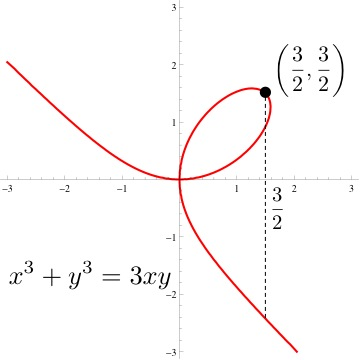
\includegraphics{./images/ch4/x3y33xy.jpg}}
\end{center}
如果用形如$y=f(x)$的函数表示这条曲线,显然会相当复杂。

设我们所要求切线的点所在的一段曲线可以表示为$y=y(x)$,带入到方程中可得
$$x^3+y^3(x)=3xy(x),$$
这个方程左右都是关于$x$的函数,于是可以考虑两边求导,然后利用求导后的
结果来推导出$y'(x)$的表达式。

[解]:将$y$视为$x$的函数,对已知方程两边关于$x$求导,可得
\ps{\b 在隐函数方程求导的结果中,允许同时包含$x$和$y$}
$$3x^2+3y^2y'=3y+3xy'\quad\Rightarrow\quad
y'=\df{x^2-y}{x-y^2},$$
带入$(x,y)=(3/2,3/2)$可得$y'(3/2)=-1$,故所求切线方程为
$$y=-x+3.$$
\hfill$\Box$

总结一下,{\it\b 由隐函数方程$f(x,y)=0$解出变量$y$关于$x$的导数大致的过程如下:
首先假设$y$为$x$的函数$y(x)$,则原方程即为
$$f(x,y(x))=0;$$
接下来两边同时关于$x$求导,然后利用求导后的方程解出$y'_x$。}

{\bf 补充例题:}\ps{下面几个例子都来自KD教材}

{\bf 例:}设$y=y(x)$是由方程$y^2=x^2-\cos y$所确定的隐函数,求$y''(x)$。

\begin{center}
	\resizebox{!}{6cm}{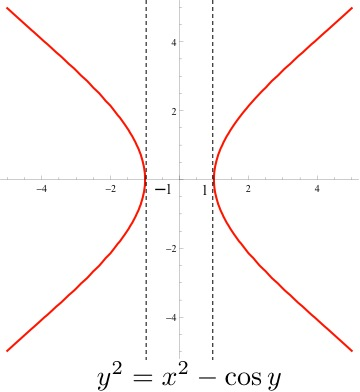
\includegraphics{./images/ch4/y2x2-cosy.jpg}}
\end{center}

{\bf 例:}求函数$y=(x^2+1)\sqrt[3]{(x-2)^2(x^2+x)}$的导数。

{\bf 例:}设$x^2+xy+y^2=1$,则
$$y'=-\df{2x+y}{x+2y},\quad y''=-\df6{(x+2y)^3}$$
$$y'''=-\df{54x}{(x+2y)^5}$$
$x+2y=0$恰好与经过角度旋转(逆时针$\pi/6$)的椭圆的交点出切线与$y$轴平行。

\begin{shaded}
	下面这道题有很多精彩的解法,这是其一:
	
	{\bf 例:}证明椭圆上任一点处的法线平分该点与两个焦点的连线所夹角。

	[提示]:{\it 如图
	\begin{center}
		\resizebox{!}{5cm}{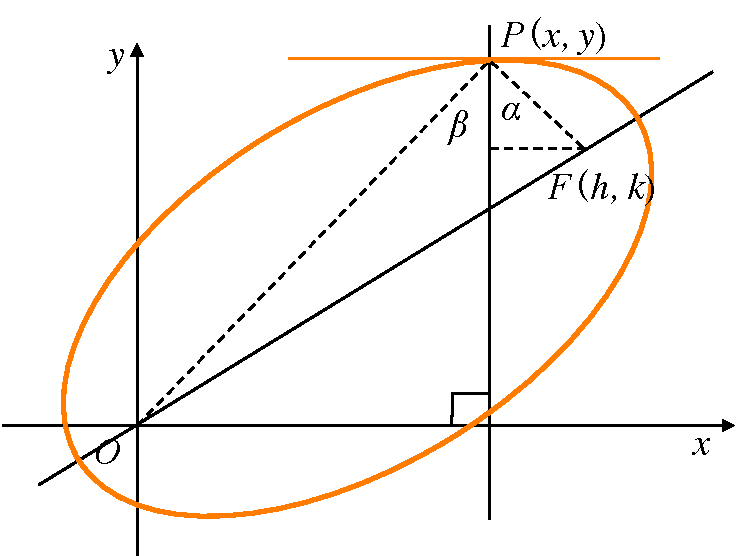
\includegraphics{./images/ch4/rollEc.pdf}}
	\end{center}
	只需证明上半椭圆上任一点有此性质即可。通过旋转椭圆,总可以是点$P(x,y)$处的切线为水平的,
	即$y'(x)=0$。
	此时,设椭圆的两个焦点分别为$(0,0)$和$(h,k)$,则由椭圆的几何性质,有
	$$\sqrt{x^2+y^2}+\sqrt{(x-h)^2+(y-k)^2}=L,$$
	其中$L$为某个确定的值。两端同时对$x$求导,并带入$y'(x)=0$,可得
	$$\df{x}{\sqrt{x^2+y^2}}=\df{h-x}{\sqrt{(x-h)^2+(y-k)^2}}.$$
	由图上不难看出该式也即$\sin\alpha=\sin\beta$,即证。}
		
[又解]:
设椭圆为$\frac{x^2}{a^2}+\frac{y^2}{b^2}=1$,左右焦点分别为$F_1,F_2$,椭圆上任意一点$P(x_0,y_0)$。
$P$点处法线平分$\angle F_1PF_2$的充分必要条件为$P$点处切线平分$\angle F_1PF_2$的外角。
$\frac{x^2}{a^2}+\frac{y^2}{b^2}=1$两边同时关于$x$求导,有
$$\frac{2x}{a^2}+\frac{2yy’}{b^2}=0,$$
得
$$y’=-\frac{b^2x}{a^2y}$$
所以$P$处的切线斜率$k=-\frac{b^2x_0}{a^2y_0}$。
又$\angle 1,\angle 2\in(0,\pi/2)$,且
$$\tan\angle 1=-\frac{b^2y_0}{a^2y_0}-\frac{y_0}{x_0}-c=\frac{b^2}{cy_0},$$
同理$\tan\angle 2= \frac{b^2}{cy_0}$,
故$\angle 1=\angle 2$。

\end{shaded}

\subsection{参数方程求导法则}

参数方程也是一种常见的表示几何对象(例如平面曲线)的方式,而且和
隐函数方程具有一样强的表示能力。平面曲线的参数方程通常形如:
$$
	\left\{\begin{array}{l}
		x=x(t),\\
		y=y(t),
	\end{array}\right.\;t\in [a,b].
$$

在此,我们假设$x(t),y(t)$均可导,来考虑一下$y$关于$x$的导数。
参考上一节中的“形式化”推导方法,可以发现
\begin{thx}
	$${\b y'(x)}=\df{\d y}{\d x}=\df{\d y}{\d t}\df{\d t}{\d x}
	=\df{\df{\d y}{\d t}}{\df{\d t}{\d x}}={\b \df{y'(t)}{x'(t)}}$$
\end{thx}
给出某个点$(x,y)$对应的$t$,利用上式右端的公式就可以求出在该点处
$y$关于$x$的导数(或者说切线斜率)了——当前不要忘记一个必要的前提,
$x'(t)\ne 0$\ps{事实上,如果将$x$视为自变量,显然必须要求$x(t)$是可逆的,
也即$x'(t)\ne 0$}。

不妨再进一步,考虑$y$关于$x$的二阶导数。
\begin{thx}
	\begin{align*}
		{\b y''(x)}&=\df{\d^2y}{\d x^2}=\df{\d}{\d x}y'(x)
		=\df{\d}{\d x}\left(\df{y'(t)}{x'(t)}\right)
		=\df{\d}{\d t}\left(\df{y'(t)}{x'(t)}\right)\cdot\df{\d t}{\d x}\\
		&=\df{y''(t)x'(t)-y'(t)x''(t)}{[x'(t)]^2}\cdot\df1{x'(t)}
		={\b \df{y''(t)x'(t)-y'(t)x''(t)}{[x'(t)]^3}}
	\end{align*}
\end{thx}

掌握这种推导方法,对于更好地推导计算各类求导公式是非常重要的。

{\bf 例:}求抛物线$x=y^2$在$(1,1)$和$(4,-2)$处的切线方程。

{\bf 例:}已知$\left\{\begin{array}{l}x=t-\sin t\\
y=1-\cos t\end{array}\right.$,求$y''(x)$。
\begin{center}
	\resizebox{!}{3.2cm}{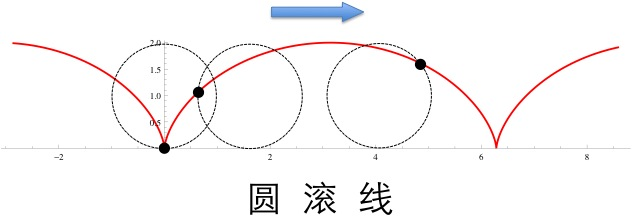
\includegraphics{./images/ch4/sphereRoll.jpg}}
\end{center}

{\bf 例:}设$\left\{\begin{array}{l}x=f\,'(t)\\ y=tf\,'(t)-f(t)
\end{array}\right.$,求$\df{\d^2y}{\d x^2}$,其中$f\,''(x)$存在且不为零。

{\bf 例:}由$x^2+xy+y^2=1$的参数方程
$$x=\df2{\sqrt3}\cos t,\quad y=\sin t-\df1{\sqrt3}\cos t$$
求$y$关于$x$的一至三阶导数。
[提示]:
$$y'_x=-\df{\sqrt3}2\cot t-\df12$$
$$y''_{xx}=-\df34\csc^3t$$
$$y'''_{xxx}=-\df{9\sqrt3}8\df{\cos t}{\sin^5t}$$
事实上,$t=\arccos\df{\sqrt3}2x$,当$\sin t\ne0$,也即$t\ne2k\pi-\df{\pi}6$
时以上导数才有意义。

\begin{shaded}
	{\bf 例:}{\kaishu Archimedes螺线}
	$\rho=a\theta$与双曲螺线$\rho=a/\theta$相交处相互垂直。

	\begin{center}
		\resizebox{!}{8cm}{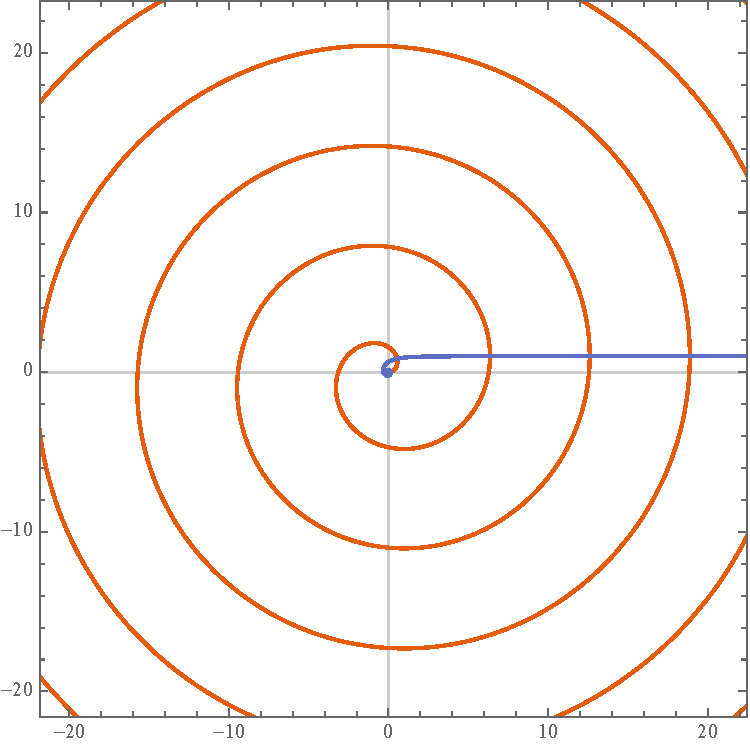
\includegraphics{./images/ch4/arCurve.pdf}}
		
		{\kaishu$\rho=\theta$和$\rho=1/\theta$\quad($\theta\in(0,10\pi)$)
		
		两曲线的交点为$\theta(k)=-k\pi+\sqrt{k^2\pi^2+1},(k\in\mathbb{N})$
		
		但是注意到只有当$k=0$时,曲线交点处的$\theta$值才对两个函数来说才是相同的,
		
		因此,两条曲线真正意义上的交点只有$\theta=1$
		}
	\end{center}
	
	[提示]:两曲线的参数方程分别为
	$$
	\left\{\begin{array}{l}
		x=a\theta\cos\theta\\
		y=a\theta\sin\theta
	\end{array}\right.
	\quad\quad\quad
	\left\{\begin{array}{l}
		x=\df{a}{\theta}\cos\theta\\
		y=\df{a}{\theta}\sin\theta
	\end{array}\right.
	$$
	相应的曲线斜率分别为
	$$y'_x=\df{\sin\theta+\theta\cos\theta}{\cos\theta-\theta\sin\theta}
	\quad\quad\quad
	y'_x=-\df{\theta\cos\theta-\sin\theta}{\theta\sin\theta+\cos\theta}
	$$
	显然$\theta=1$时二者的乘积为$-1$,这意味着两条曲线在交点处垂直!
	
	{\bf 问:}$k\ne0$时,从图像上看两条曲线也是相互垂直的,如何证明呢?
\end{shaded}

\begin{ext}
	{\centering\bf 课后作业}
	
	\begin{enumerate}  
	  \item 对下列函数,求$y''(x)$
	  \begin{enumerate}[(1)]
	    \item $y=\tan(x+y)$;
	    \item $y=1+xe^y$。
% 	    \item $x=t(1-\sin t),\;y=t\cos t$。
	  \end{enumerate}
	  \item 求曲线$\left\{\begin{array}{l}
	  	x=\df{3t}{1+t^2},\\ y=\df{3t^2}{1+t^2}.
	  \end{array}\right.$在$(0,0)$和$\left(\df32,\df32\right)$
	  处的切线方程。
	  \item 已知$\left\{\begin{array}{l}
	  	x=e^x\cos t\\ y=e^x\sin t
	  \end{array}\right.$,求$\left.\df{\d y}{\d x}\right|_{t=\frac{\pi}2}$
	  和$\left.\df{\d^2 y}{\d x^2}\right|_{t=\frac{\pi}2}$。
	  \item (选作)设$x(t),y(t)$均三阶可导,试给出$y'''_{xxx}$关于$t$的表达式。
	  \item (选作)设曲线的极坐标方程为$\rho=\rho(\theta)$,求其对应的直角指标
	  方程$y=y(x)$相关的导数$y'_x$和$y''_{xx}$关于$\theta$的表达式。
	\end{enumerate}
\end{ext}

\section{相关变化率}

{\it 变化率}可以定义为,一个变量随另一个变量变化过程中,相对于后者发生变化的速率,或者
二者的相关的变化量的比值。对于连续变化的函数而言,导数所刻画的正是函数值关于自变量
的变化率。常见的变化率的例子包括:

\begin{itemize}
  \setlength{\itemindent}{1cm}
  \item {\it 曲线的斜率}:函数值关于自变量的变化率 
  \item {\it 速度}:位移关于时间的变化率 
  \item {\it 密度}:质量关于体积的变化率 
  \item {\it 电流强度}:电量关于时间的变化率 
  \item {\it 边际收益}:收益关于投入的变化率 
  \item 等等{\ldots\ldots} 
\end{itemize}

在现实问题中,许多变量之间都存在着千丝万缕的联系,从它们基本的数量关系出发,
往往能够进一步去研究它们的变化率(导数)之间的关系。

在学习掌握了导数的概念和计算方法之后,本节所讨论的相关变化率问题是对导数
的一个初步应用。

{\bf 例:}有一深度$8$m,上底直径$8$m的圆锥形容器,
以$4$m$^3$/min的速率向其中注水,当容器中水深$5$m时,水面上升的速度是多少?

{\bf 例:}甲乙两船分别向南和向东航行。在初始时刻,甲船恰位于乙船北方
$40$km处,后来在某一时刻测得甲船向南航行了20km,此时速度为15km/h;
乙船向东航行了15km,此时速度为25km/h。问该时刻两船是在相互靠近还是远离,
二者的相对速度是多少?

% {\bf 例:}质点$P$沿抛物线$x=y^2(y>0)$移动。$P$的横坐标$x$的变化速度为$5$cm/s。
% 当$x=9$cm时,点$P$到原点的距离的变化速率是多少?
% 
% [提示]:
% $$\df{\d}{\d t}\sqrt{x^2+y^2}=\left(\sqrt{x^2+x}\right)'_xx'_t
% =\df{5(2x+1)}{\sqrt{x^2+x}}$$
% 代入$x=9$,可得其值为$\df{95}{6\sqrt10}$(cm/s)

{\bf 例:}钟表的时针和分针长度分别为$a$(cm)和$b$(cm),求$12:20$分,两针端点分离的速率。

[提示]:两针的夹角变化速率$\theta'_t=\df{\pi}{30}-\df{\pi}{360}
=\df{11}{360}\pi$(弧度/分钟)。12:20时,$\theta=\df23\pi-\df{\pi}{18}
=\df{11}{18}\pi$。利用余弦定理
$$s^2=a^2+b^2-2ab\cos\theta$$
答案$0.38$(cm/min)

% {\bf 例:}圆形广场中央立着高度为$h$的灯柱,灯$A$位于灯柱顶端。
% 广场上任一点$P$处的照明强度$I$与该点到灯的距离的平方成反比,与光线与灯柱的
% 夹角的余弦成正比。一个人从距离灯柱$x$m处以速度$v$m/s沿径向离开柱子,求
% 其脚部的光照强度关于时间的变化率。
% 
% [提示]:由已知
% $$I=k\df{h}{(x^2+h^2)^{\frac32}}.$$
% 从而
% $$I'_t=I'_xx'_t=vI'_x=-\df{xvkh}{(x^2+h^2)^{\frac52}}$$

{\bf 例:}一个长度为$l$的杆,一段连接半径为$r$的转轮,一段位于$x$轴上。转轮的中心
位于原点,以每分钟$m$转的速度逆时针旋转,求:杆位于$x$轴上的一端的运动速率。

[提示]:如图
\begin{center}
	\resizebox{!}{4cm}{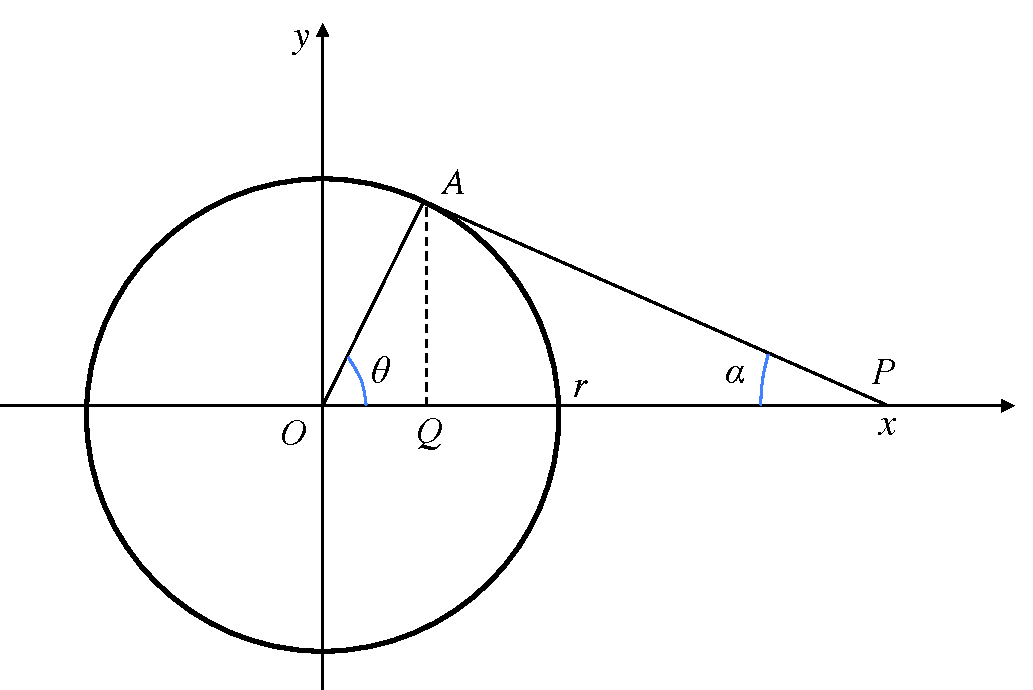
\includegraphics{./images/ch4/rollbar.pdf}}
\end{center}
$$\sin\theta=\df{|AQ|}r,\quad \sin\alpha=\df{|AQ|}{l}$$
从而$\sin\alpha=\df rl\sin\theta$,进而$\alpha=\arcsin\left(
\df rl\sin\theta\right)$。
$$x=r\cos\theta+l\cos\alpha=r\cos\theta+l\cos
\left[\arcsin\left(\df rl\sin\theta\right)\right]$$
$x'_t=x'_{\theta}\theta'_t=2m\pi x'_{\theta}$,其中
$$x'_{\theta}
% =-r\sin\theta-r^2\sin\theta\cos\theta
% \df1{\sqrt{l^2-r^2\sin^2\theta}}
=-r\sin\theta\left(1-\df{r\cos\theta}{\sqrt{l^2-r^2\sin^2\theta}}\right)$$

{\bf 例:}边长$s$的正方体冰块在空气中融化,已知冰块的融化速度(体积减少速度)
与其表面积成正比,比例系数为$k(k>0)$。假设冰块融化的过程中始终保持正方体形状。经过
一个小时,其体积减少了四分之一,求其完全融化需要的时间。

[提示]:设冰块体积为$V(t)$,由已知其融化速度为
$$V'(t)=-k(6s^2).$$
又$V=s^3$,故
$$V'(t)=3s^2s'(t).$$
从而可得$s'(t)=-2k$,解得$s=-2kt+s(0)$。令$t=1$,可得$s(1)-s(0)=-2k$。

注意到$s$递减的速度与$t$无关,故冰块完全融化需要的时间
$$T=\df{s(0)}{2k}=\df{s(0)}{s(0)-s(1)}=\df1{1-\df{s(1)}{s(0)}}.$$
其中
$$\df{s(1)}{s(0)}=\left[\df{V(1)}{V(0)}\right]^{\frac13}=
\left(\df34\right)^{\frac13}\approx0.91(h)$$
代入前式计算可得$T\approx11(h)$

类似本节的示例都可以说是微积分的应用,对于这类应用问题,在解题时一般可以参考如下
的步骤:
\begin{thx}
	{\bf 求解应用题的一般步骤}
	\begin{enumerate}
	  \setlength{\itemindent}{1cm}
	  \item {{\it 画图:}}理解题意,画出示意图
	  \item {{\it 定义变量:}}给出相关变量的数学表示
	  \item {{\it 建立数量关系:}}根据已知,建立方程
	  \item {{\it 数学推导:}}例如方程两边求导(或者积分)
	  \item {{\it 求得结果:}}整理推导后的结果,得出解答
	\end{enumerate}
\end{thx}

\begin{shaded}
	{\bf 万有引力定律的推导}
	
	关于变化率和相关变化率最好的实例是Newton从Kepler三定律推导出万有引力定律的过程。
	下面的推导过程较长,能够看完并且理解,相信也是对导数这一章知识掌握情况一种很好的测试。

	在牛顿的工作之前,德国天文学家、物理学家和数学家Johannes Kepler(1571-1630)
	通过多年的天文观察,得到所谓的{\it 行星运动三大定律}——这三大定律使Kepler
	赢得了“天空立法者”的美名:
	\begin{enumerate}
	  \item {\it 轨道定律:}所有行星分别都运行在椭圆轨道上,其对应的“太阳”位于
	  椭圆的一个焦点上
	  \item {\it 面积定律:}在同样的时间内,行星{\it 向径(极径)}(即由“太阳”位置
	  指向行星位置的向量)在轨道平面上扫过的面积相等
	  \item {\it 周期定律:}行星的公转周期的平方与它同太阳最远距离的立方成正比 
	\end{enumerate}
	
	\begin{center}
		\resizebox{!}{4cm}{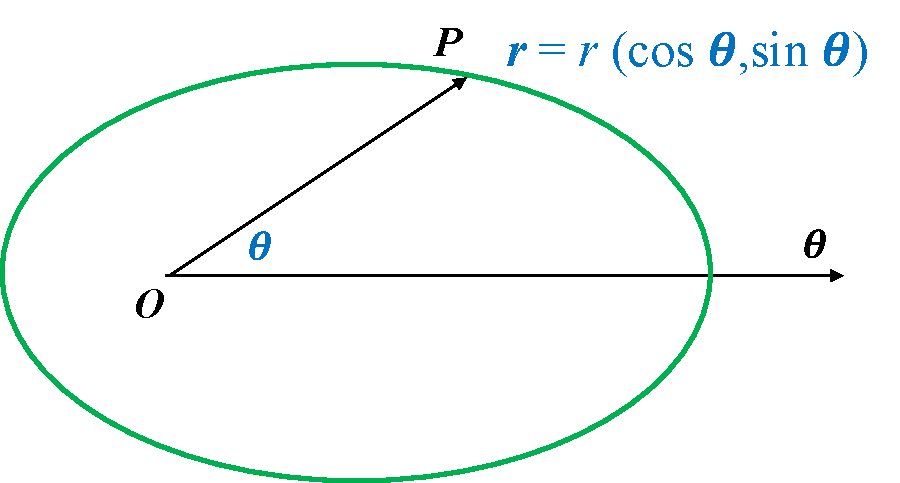
\includegraphics{./images/ch4/Kepler.pdf}}
	\end{center}
	
	如图,绿色曲线为行星的椭圆轨道,极坐标系的原点$O$表示“太阳”的位置,点$P$为行星的位置。
	椭圆的极坐标方程为
	$$r=\df{p}{1-e\cos\theta},$$
	其中:
	\begin{itemize}
	  \item {\it 焦参数}:$p=\df{b^2}a$
	  \item {\it 离心率}:$e=\sqrt{1-\df{b^2}{a^2}}$
	  \item $a,b$分别为椭圆的半长轴和半短轴长度
	\end{itemize}
	
	在$t$时刻,行星的位置可用其向径来表示(注:在印刷体中,向量默认使用粗体字母表示,在手写体
	中,则使用在字母上方画箭头的记号来表示):
	$$\bm{r}(t)=r(t)(\cos\theta,\sin\theta),$$
	其中:
	\begin{itemize}
	  \item $r(t)=|\bm{r}(t)|$($|\bm{r}|$表示向量$\bm{r}$的模,
	  或者说,长度)为向径的长度,也即行星到太阳的{\it 距离}
	  \item $\theta=\theta(t)$如图所示,为当前位置对应的{\it 极角}
	  \item 记$\bm{r}_0=(\cos\theta,\sin\theta)$为$\bm{r}(t)$对应的
	  {\it 单位向量,也称为方向向量}
	\end{itemize}
	
	根据Newton第二定律,行星所受的力(注:对向量求导等价于对其每个分量分别求导,
	例如:$\bm{r}=(x(t),y(t))$,则$\bm{r}'_t=(x'_t,y'_t)$)
	\begin{align}
		\bm{F}&=m\bm{a}=m\bm{r}''_{tt}\notag\\
		&=m\left(\df{\d^2(r\cos\theta)}{\d t},\df{\d^2(r\sin\theta)}{\d
		t}\right)\notag\\
		&=m((r''-r\omega^2)\cos\theta-(2r'\omega+r\omega')\sin\theta,
		(2r'\omega+r\omega')\cos\theta+(r''-r\omega^2)\sin\theta)\notag\\
		&=m(r''-r\omega^2)\bm{r}_0+m\left(\df{2r'\omega+r\omega'}
		{\omega}\right)\bm{r}'_0\tag{N.1}
	\end{align}
	其中:
	\begin{itemize}
	  \item $m$为{\it 行星质量}
	  \item $\bm{a}$为行星的{\it 加速度向量}
	  \item {\it 角速度}:$\omega=\theta'_t$
	  \item {\it 径向速度(率)}:$r'=\df{\d r}{\d t}$
	  \item {\it 径向加速度(率)}:$r''=\df{\d^2 r}{\d t^2}$
	\end{itemize}
	
	记$\d A$为向径转过角度$\d\theta$所对应的椭圆面积,则
	$$\d A=\df12r^2\d\theta,$$
	由Kepler第二定律,单位时间内向径扫过的面积为常数(记为$c$),即
	$$c=\df{\d A}{\d t}=\df12r^2\omega.\eqno{(\mbox{N}.2)}$$
	
	记行星的公转周期为$T$,则经过$T$时间向径扫过的面积恰为整个椭圆的面积$\pi ab$,
	也即
	$$\pi ab=\dint_0^T\df{\d A}{\d t}\d t=cT=\df12r^2\omega T,$$
	由此可解出
	$$r^2\omega=\df{2\pi ab}T.$$
	
	式(N.2)两边求导,可得
	% \ps{事实上,若记行星的公转周期为$T$,容易解得$r^2\omega=\df{2\pi ab}T$}
	$$0=(r^2\omega)'=r(2r'\omega+r\omega'),$$
	由此可见(N.1)式中的第二部分恒为零,从而
	$$\bm{a}=\bm{r}''_{tt}=(r''-r\omega^2)\bm{r}_0,$$
	这表明{\it 行星在任一点处的加速度方向(也即受力方向)是沿着其向径方向,或者
	是与其和“太阳”连线相一致的}!
	
	下面回到椭圆方程,其可以改写成
	$$p=r(1-e\cos\theta),$$
	两边求二阶导数,可得
	\begin{align}
		0&=p''=r''-e(r^2\cos\theta)''\notag\\
		&=(r''-r\omega^2)(1-e\cos\theta)+r\omega^2\notag\\
		&=\df{r''-r\omega^2}rp+r\omega^2\notag
	\end{align}
	于是
	$$r''-r\omega^2=-\df{(r^2\omega)^2}{r^2p}=-4\pi^2\df{a^3}{T^2r^2}$$
	
	根据Kepler第三定律,$\df{a^3}{T^2}$为常数,记太阳的质量为$M$,则
	$$\bm{F}=m\bm{a}=m(r''-r\omega^2)\bm{r}_0
	=-\left(\df{4\pi^2a^3}{MT^2}\right)\df{Mm}{r^2}\bm{r}_0,$$
	记{\it 万有引力常数}
	$$G=\df{4\pi^2a^3}{MT^2}\approx 6.67\times 10^{-11}
	(\mbox{m}^3/\mbox{kg}\cdot\mbox{s}^2),
	$$
	也即
	$$\bm{F}=-G\df{Mm}{r^2}\bm{r}_0$$
	
	% \begin{shaded}
	
	万有引力定律说明了宇宙万物之间都存在相互的引力,且引力的作用方向在二者的连线上,
	其大小与二者的质量乘积成正比,与二者的距离平方成反比,比例系数为{\it 绝对常数}(
	即在宇宙范围内为常数,相对而言,前述推导中出现的常数如$c$,$a^3/T^2$都
	是和所处的“太阳-行星”系统相关的)。
	
	% \end{shaded}
	
	以上的论证及其结果,并不就是Newton个人所完整发现的,事实上也不是Newton最初的论证
	(发表在Newton的巨著《自然哲学的数学原理》一书上)。
	Kepler已经证明了,如果行星的轨迹是圆形,则符合万有引力定律。但如果轨道是椭圆形的,
	Kepler由于没能像Newton发明了微积分那样,拥有更合适的数学工具,因此得不出所要的结果。
	
	另一方面,Newton最初的论证,只是说明了以上规律对我们所处的“太阳-行星”系统是正确的,
	是其后的科学家进一步证实了这一规律”放之四海而皆准“,适用于从一切天体运动到微观
	世界的广泛范围,而所有后续论证的基础是大量的实验观测。例如,万有引力常数$G$的值于
	1789年由Henry Cavendish(1731-1810)利用他所发明的{\it 扭称}得出的。
	
	基于万有引力定律,诞生了一些非常著名的天文学成果,例如:
	
	\begin{itemize}
	  \item 计算出哈雷彗星的轨道和运动周期
	  \item 发现了海王星和冥王星
	  \item 解释了潮汐的起因和规律
	  \item 计算出第一、第二和第三宇宙速度,从而开启了人类航天活动的历史
	\end{itemize}
	
	利用万有引力定律,可以反向推导出Kepler的行星运动三定律。其中第二和第三定理
	的推导相对容易,下面给出由万有引力定律推导Kepler第一定律的大致过程。
	
	Newton第二定律的极坐标形式
	$$
	\left\{\begin{array}{l}
		F(r)=m(r''-r(\theta')^2)\\
		F(\theta)=m(r\theta''+2r'\theta')
	\end{array}\right.
	$$
	
	Binet公式:(参见Wikipedia关于Binet Equation的条目)
	$$F=-mh^2u^2\left(u''_{\theta\theta}+u\right)$$
	其中:$u=\df1r$,$h=\df Lm=r^2\theta'$,由角动量守恒定律,为常数。
	
	万有引力方程可以写为
	$$F=-mk^2u^2,$$
	其中$k^2=GM$(称为{\kaishu Guass常数},是一个与行星无关,而只与太阳有关的量)。综合以上
	两式,可得
	$$u''_{\theta\theta}+u=\df{k^2}{h^2},$$
	以下解方程。令$u=\xi+\df{k^2}{h^2}$,则方程化为
	$$\xi''_{\theta\theta}+\xi=0,$$
	这是一个波动方程,其解具有如下形式
	$$\xi=A\cos(\theta-\theta_0),$$
	进而
	$$r=\df1u=\df{h^2/k^2}{1+A[\cos(\theta-\theta_0)]h^2/k^2}$$
	这实质上就是椭圆的极坐标方程。
\end{shaded}

\begin{ext}
	{\centering\bf 课后作业}
	
	\begin{enumerate}  
% 	  \item 圆形广场中央立着高度为$15$米的灯柱,有一盏灯位于灯柱顶端。
% 		广场上任一点处的照明强度$I$与该点到灯的距离的平方成反比,与光线与灯柱的
% 		夹角的余弦成正比。一个人从距离灯柱$10$米处以速度$1.5$米每秒沿径向离开柱子,求
% 		其脚部的光照强度关于时间的变化率。
	  \item 质点$P$沿抛物线$x=y^2(y>0)$移动。$P$的横坐标$x$的变化速度为$5$cm/s。
		当$x=9$cm时,点$P$到原点的距离的变化速率是多少?
	  \item 垂直向上发射一枚火箭,在其起飞点100km外设置一个观察站,在观察仰角
	  为$\pi/4$时,测得仰角的增加率为$0.1$弧度每秒,求此时火车的上升速率。
	  \item 长度为$6$米的梯子靠在墙角,梯子底部距离墙角$5$米,某一时刻梯子底部开始
	  向远离墙角的方向滑动,滑动的速度为$0.2$米每秒,问
	  \begin{enumerate}[(1)]
	    \item 此时梯子顶部下滑的速度是多少?
	    \item 由梯子、墙面和地面构成的三角形的面积随时间的变化率是多少?
	    \item 梯子和地面的夹角的以怎样的速率变化?
	  \end{enumerate}
	  \item 半径为$a$的圆球渐渐沉入盛有水的半径为$b(b>a)$的圆柱形容器中,若
	  球的下降速度恒为$c$,求球浸没入水中恰好一半时,容器内水面上升的速率。
	  (提示:球冠的体积$V=\df{\pi}3(3R-H)H^2$,其中$H$为球冠的高度)
% 	  \item (选作)设曲线的极坐标方程为$\rho=\rho(\theta)$,求其对应的直角指标
% 	  方程$y=y(x)$相关的导数$y'_x$和$y''_{xx}$关于$\theta$的表达式。
	\end{enumerate}
\end{ext}

\section{微分}

计算函数的值从来都是一个简单问题,这一点大多数刚学习微积分不就的人都不会意识到。
例如一个段子:你被判了无期,假释的唯一可能是算出$\sin 1$的近似值,要求精确到小数点后
100位,而你的工具只有无限量使用的笔和纸。就你现在的知识,你觉得可能在有生之年
完成吗?或者改换一下任务,算算$\ln 3$?

数学家们显然也意识到了这个问题,在想给出了用导数刻画变化率的办法之后,
他们很快发现了它与{\it 近似计算}之间的联系。请注意,这个故事很长,本节只是开篇,
等到下一章学习了Taylor公式后才能真正告一段落。

\subsection{局部线性化和“以直代曲”}

对于任意给定的函数,如果已知它在某点的函数值,能否给出它附近其他点处的函数值,
并且尽可能精确\ps{在现实里,绝对的精确是不存在的,数学上中的计算其实也是一样}?

一个自然的想法是,用一条尽可能简单,而且易于计算函数值的曲线来近似给定的曲线,
由于没有比{\it 直线}(或者叫"{\it 线性函数"})更简单的函数形式,因此它就成了第一个
尝试的对象,对应的想法被称为“{\it 以直代曲}”\ps{后面我们还将学习它的“高级版本”——“以曲代曲”},
数学上这样定义:
\begin{thx}
	设已知函数$f(x)$在$x_0$附近有定义,记$\Delta y=f(x_0+\Delta x)-f(x_0)$,
	如果存在某个与$\Delta x$无关的常数,使得
	$$\Delta y=A\cdot\Delta x+\circ(\Delta x),\;(\Delta x\to 0),$$
	则称$f(x)$可以被以直代曲,或者更规范的说法是{\bf $f(x)$在$x_0$处可微},还有
	一种说法是$f(x)$在$x_0$附近可以“{\bf 局部线性化}”。此时,我们称
	$$\left.\d y\right|_{x=x_0}=A\cdot\Delta x$$
	为{\bf $f(x)$在$x_0$处的微分},当$x$是自变量时,一般认为$\d x=\Delta x$,故
	上式一般就记为:
	$$\left.\d y\right|_{x=x_0}=A\cdot\d x.$$
\end{thx}

\begin{center}
	\resizebox{!}{6cm}{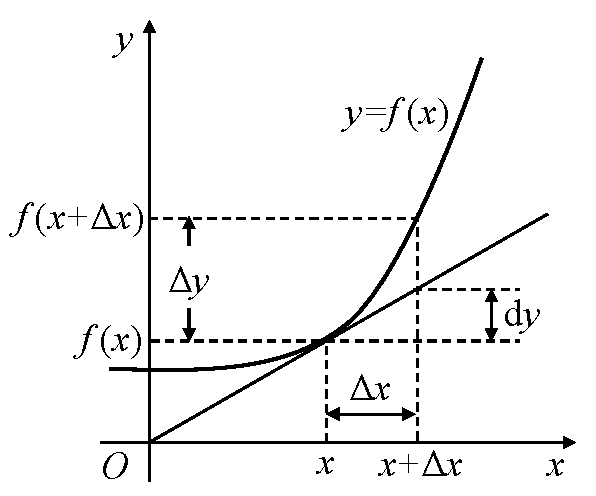
\includegraphics{./images/ch4/dy.pdf}}

	\it $f(x)$在$x_0$可微,意味着在$x_0$附近,$f(x)$可以近似地表示为一个线性函数: 
	$$f(x)\approx y= f(x_0)+f\,'(x_0)(x-x_0)$$
\end{center}

不难看出,$f(x)$在$x_0$可微时,用于和$f(x)$近似的线性函数所对应的
恰好就是$y=f(x)$在$x_0$处的切线,因此$A$就是切线的斜率,换句话说,
$A=f'(x_0)$。下面我们从代数上推导一下可微和可导的关系。

\begin{thx}
	{\bf 可导与可微的关系:}$f(x)$在$x_0$可微与$f(x)$在$x_0$可导等价,且
	$$\d y =f'(x_0)\d x.$$
\end{thx}

[证]:设$f(x)$在$x_0$可微,则存在$A$,使得
$$f(x)-f(x_0)=A(x-x_0)+\circ(x-x_0),\;(x\to x_0),$$
该式进行恒等变形可得
$$\df{f(x)-f(x_0)}{x-x_0}=A+\circ(1),\;(x\to x_0),$$
也即
$$A=\lim\limits_{x\to x_0}\df{f(x)-f(x_0)}{x-x_0},$$
故$f(x)$在$x_0$可导,且$f'(x)=A$。

又,设$f(x)$在$x_0$可导,则有
$$f'(x_0)=\lim\limits_{x\to x_0}\df{f(x)-f(x_0)}{x-x_0},$$
从而易得
$$\lim\limits_{x\to x_0}\df{f(x)-f(x_0)
-f'(x_0)(x-x_0)}{x-x_0}=0,$$
故
$$f(x)-f(x_0)-f'(x_0)(x-x_0)=\circ(x-x_0),\;(x\to x_0),$$
也即
$$f(x)-f(x_0)=f'(x_0)(x-x_0)+\circ(x-x_0),\;(x\to x_0),$$
由此可知$f(x)$在$x_0$可微,且
$$\d y =f'(x_0)\d x.$$
\hfill$\Box$

导数也做{\it 微商},有了上面的定理不难理解这是为什么。

{\bf 例:}设$f(x)=x^3+2x^2-3x+6$,求$\d f(x)$和$\d f(x)|_{x=1}$,
并求其在$(1,6)$处的{\b 局部线性化函数$L(x)$}。

\subsection{微分的运算法则}

了解了导数和微分之间的密切联系,就可以很容易地有各种求导法则
推出下面的微分运算法则:

\begin{thx}
	{\bf 微分与四则运算:}设$u(x),v(x)$可微(导),则
	\begin{enumerate}[(1)]
	  \setlength{\itemindent}{1cm}
	  \item $\d (u\pm v)=\d u\pm \d v$
	  \item $\d(uv)=v\d u+u\d v$
	  \item $\d\df uv=\df{v\d u-u\d v}{v^2}$
	\end{enumerate}
	
	{\bf 复合函数的微分:}设$y=g(u),u=f(x)$均可微,
	则$y=g[f(x)]$可微,
	$$\d y=g'(u)\d u=g'(u)f'(x)\d x$$		
\end{thx}

从形式上看,复合函数的微分运算规则更有链式法则的“环环相扣”的味道,
事实上,对于一阶的微分运算(与一阶导数对应),我们不必关心每个
变量究竟是因变量还是自变量,或者是中间变量,从结果上看都具有类似
$$\d y=y'_x\d x$$
的形式,比如在上面的结论中
$$\d y=f'(u)f'(x)\d x,$$
其中的$f'(u)g'(x)$就是$y$关于$x$的导数$y'_x$。
这种性质非常有利于我们计算各种(一阶)微分,被称为{\it 一阶微分的
形式不变性。}\ps{高阶微分不具有此性质}

{\bf 例:}求函数$y=e^{2x-1}\sin x$的微分。

[解]:
\begin{align*}
	\d y
	&=\d(e^{2x-1}\sin x)
	=e^{2x-1}\d\sin x+\sin x\d e^{2x-1}\\
	&=e^{2x-1}\cos x\d x+\sin x 2e^{2x-1}\d x
	=(\cos x+2\sin x)e^{2x-1}\d x.
\end{align*}
\hfill$\Box$

\subsection{微分的应用}

有了微分这种对函数的局部近似,我们就可以对一些已知函数值附近的函数值进行
有效的逼近,或者,对于可能产生的计算误差进行分析。

{\bf 例:}\ps{同济教材例7}
有一批半径为$1$cm的球,为了提高球面的光洁度,准备镀上一层铜,
厚度为$0.01$cm,试估计每只球需要的用铜量(铜的密度为$8.9$g/cm$^3$)。

[提示]:所需的铜量
$$M=8.9\cdot\Delta V,$$
其中$\Delta V$为镀铜前后球的体积差,利用微分进行近似,
$$\Delta V\approx \d V=\d\left(\df43\pi R^3\right)
=4\pi R^2\d R=4\pi R^2\Delta R,$$
将$R=1,\Delta R=0.01$带入计算,可得
$$\Delta V\approx 0.13(\mbox{cm}^3),$$
最终每个球所需铜量约为$1.16$g。

同样是这个例子,我们换一个角度来提问:

{\bf 例:}如果上述的球体在加工时,半径最大允许$0.01$cm的误差,
估计一下球的体积的绝对误差和相对误差分别有多大。

[提示]:利用微分进行估计
$$\Delta V\approx \d V=\d\left(\df43\pi R^3\right)
=4\pi R^2\d R=4\pi R^2\Delta R,$$
将$R=1,\Delta R=0.01$带入计算,可得
$$\Delta V\approx 0.13(\mbox{cm}^3),$$
注意到$\Delta$关于$\Delta R$是严格单调的,故以上就是所求的
体积的{\it 绝对误差}的近似值。进而相对误差
$$e_r=\df{\Delta V}{V}\approx 3\df{\Delta R}{R}=3\%.$$

现实中“以直代曲”的例子:桥梁的设计

\begin{center}
	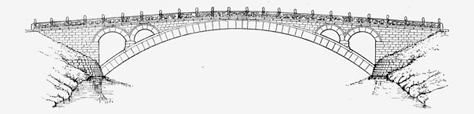
\includegraphics[width=0.75\textwidth]{./images/ch2/archBridge-1.jpg}
	
	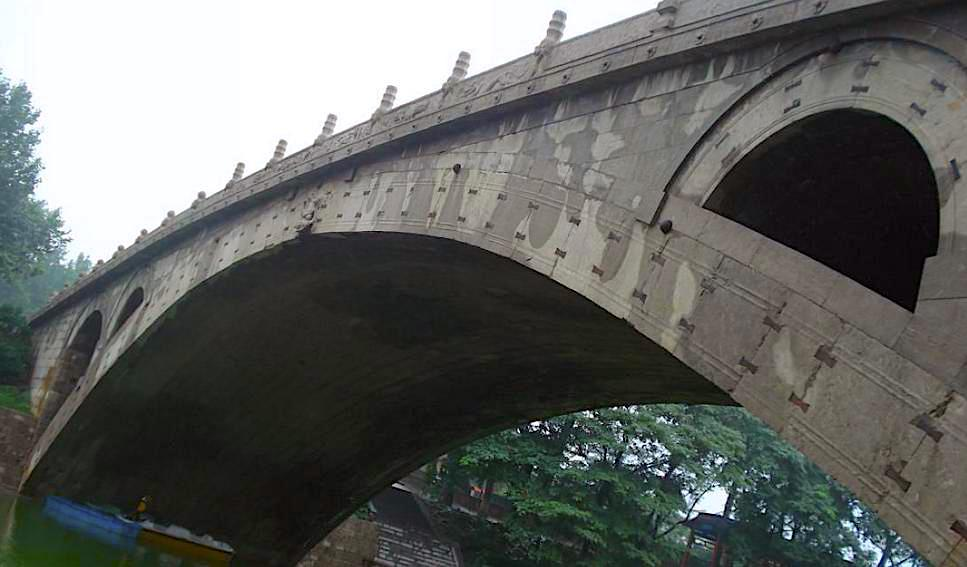
\includegraphics[width=0.75\textwidth]{./images/ch2/zhaozhouqiao.jpg}
	
	\it 赵州桥
\end{center}

\begin{ext}
	{\centering\bf 课后作业}
	
	\begin{enumerate}  
	  \item 设$y=x^3-2x$,
	  \begin{enumerate}[(1)]
	    \item 计算在$x=2$处当$\Delta x$分别为$1,\;0.1,\;
	  	0.01$时的$\Delta y$和$\d y$;
	    \item 写出$x=2$时$y$的微分表达式。
	  \end{enumerate}
	  \item 已知$2^{xy}=x-y$,求$\d y|_{x=0}$。
	  \item 同济教材习题2-5:4
	  \item 设
	  $f(x)=\lim\limits_{t\to\infty}t^2
	  \left[e^{x+\frac2t}-e^x\right]\sin\df xt$,求$\d f(x)$。
	  \item 已知当$h\to 0$时,
	  $$f(x+2h)-f(x)=h\sqrt{x^2+2x}+\circ(h),$$
	  求$\d\left[f\left(\df1x\right)\right]$。
	  \item (选作)设$a>0$,$|x|<<a$(表示$|x|$远远小于$a$),证明近似公式
	  $$\sqrt[n]{a^n+x}\approx a+\df{x}{na^{n-1}}.$$
	\end{enumerate}
\end{ext}

\section{小结}

导数即函数的{\it 变化率}\ps{变化率的另一种定义是单位自变量对应的函数改变量,例如:
单位水平位移对应的垂直位移——即斜率(或坡度),单位长度对应的质量——即线密度},
或者说是函数值的改变量关于自变量的改变量的比率,
代数上将其定义为自变量为特定取值时以上比率的极限。现实世界里的速度、
斜率和密度等都可以用导数来加以描述。

本章的重点是{\it 导数的计算},其中涉及众多{\it 基本初等函数的求导公式}和{\it 四则运算、
复合运算、函数逆运算的求导法则},这些都必须熟练掌握,作到{\it “倒背如流”}。
高阶导数的计算是本章的一个难点,正确地进行归纳和使用Leibniz{\it 公式}常常
是解题的关键。

微分的概念比较抽象,但就一元函数而言,可导和可微是等价的,因此可以简单
地将微分理解为求导的另一种形式——虽然两者有着不同的解释和物理、几何意义。
微分的计算公式都有等价的求导公式。

本章中有专门的一节讨论与导数相关的应用问题——{\it 变化率与相关变化率},
这些问题看似平常,却常常称为学习掌握的难点,正确解题的关键在于
如何正确用数学的符号和语言去描述实际问题,用更专业的话来说,
就是如何做好数学建模。

\newpage

\section*{作业参考解答}
% \addcontentsline{toc}{section}{作业参考解答}

\begin{center}
	\bf 1.2 导数的概念
\end{center}

\bigskip

1.已知$f(x)=\left\{\begin{array}{ll}
2e^x+b,& x\leq0\\ ax+\sin x,& x> 0
\end{array}\right.$
试确定$a,b$的值,使得$f(x)$在$x=0$处可导。

[解]:$f(x)$在$x=0$处可导,故必连续,从而
$$f(0-0)=2+b=f(0+0)=0,\quad\Rightarrow \quad b=-2.$$
又
$$f'_-(0)=(2e^x+b)'|_{x=0}=2.$$
$$f'_+(0)=\limx{0+}\df{ax+\sin x-(2+b)}{x}
=a+\limx{0+}\df{\sin x}x=a+1.$$
故要使$f(x)$在$x=0$处可导,必有$2=a+1$,从而$a=1$。
\hfill$\Box$

\bigskip

2.证明:曲线$xy=a^2$上任一点处的切线与两坐标轴构成的三角形面积不变。

[解]:在已知曲线上任一点$(x_0,y_0)$处,切线斜率为
$$k=\left(\df{a^2}{x}\right)'_{x=x_0}=-\df{a^2}{x_0^2}.$$
于是过该点的切线为
$$y=y_0-\df{a^2}{x_0^2}(x-x_0).$$
其在$x$轴和$y$轴上的截距分别为(注意:$y_0=\df{a^2}{x_0}$)
$$X=\df{y_0x_0^2}{a^2}+x_0=2x_0,\quad
Y=y_0+\df{a^2}{x_0^2}x_0=2y_0.$$
故该切线与两坐标轴所围三角形面积为
$$S=\df12XY=2x_0y_0=2a^2.$$
由$(x_0,y_0)$的任意性,即证。\hfill$\Box$

\bigskip

3.讨论函数
$y=\left\{\begin{array}{ll}
	x^2\sin\df1x,& x\ne0;\\ 0, & x=0.
\end{array}\right.$
在$x=0$处的连续性、可导性以及导函数的连续性。

[解]:当$x\ne 0$时,
$$f'(x)=2x\sin\df1x-\sin\df1x.$$
当$x=0$时,
$$f'(0)=\limx0\df{x^2\sin\df1x-0}{x-0}=0.$$
由此可知$f(x)$在$x=0$处可导,且连续。

又因为
$$\limx02x\sin\df1x=0,\quad \limx0\sin\df1x\mbox{不存在},$$
故$\limx0f'(x)$不存在。由此可知$f(x)$的导函数在$x=0$处不连续。\hfill$\Box$

\bigskip

4.设对任意$x\in\mathbb{R}$,均有$f(x+2)=f(x)$,已知$f'(0)=1$,
证明$f(x)$在$x=2$可导,并求$f'(2)$。

[解]:因为$f(x+2)=f(x)$,故
$$\lim\limits_{\Delta x\to0}\df{f(2+\Delta x)-f(2)}{\Delta x}
=\lim\limits_{\Delta x\to0}\df{f(\Delta x)-f(0)}{\Delta x}
=f'(0)=1,$$
由此即知$f(x)$在$x=2$可导,且$f'(2)=1$。
\hfill$\Box$

\bigskip

5.已知曲线$y=f(x)$和曲线$y=\sin x$在原点相切(即二者的切线相同),
求$\limx0\df{f(3x)}x$。

[解]:曲线$y=f(x)$和曲线$y=\sin x$在原点相切,故
$$f(0)=\sin 0=0,\quad f'(0)=(\sin x)'|_{x=0}=1.$$
于是
$$\limx0\df{f(3x)}x=3\limx0\df{f(3x)}{3x}=3f'(0)=3.$$
\hfill$\Box$

\bigskip

6.已知$f'(a)f(a)\ne 0$,求
$\limx0\left[\df{f(a+x)}{f(a)}\right]^{\frac1{\sin x}}.$

[解]:
\begin{align*}
	\mbox{原式}&=\limx0\left[1+\df{f(a+x)-f(a)}{f(a)}\right]^{\frac1{\sin x}}\\
	&=\limx0\left[1+\df{f(a+x)-f(a)}{f(a)}\right]^{\frac{f(a)}{f(a+x)-f(a)}
	\frac{f(a+x)-f(a)}{f(a)}\frac1{\sin x}}\\
	&=\left\{\limx0\left[1+\df{f(a+x)-f(a)}{f(a)}\right]^{\frac{f(a)}{f(a+x)-f(a)}}\right\}
	^{\limx0\frac{f(a+x)-f(a)}x\frac{x}{\sin x}\frac1{f(a)}}\\
	&=e^{\frac{f'(a)}{f(a)}}
\end{align*}
\hfill$\Box$

\bigskip

7.设对任意$x,y\in\mathbb{R}$,有
$$f(x+y)=f(x)+f(y)+x^2y+xy^2,$$
且当$x\to0$时$f(x)$与$x$是等价无穷小,证明$f(x)$处处可导,并求其导函数。

[解]:令$x=y=0$,由已知等式可得$f(0)=0$。

对任意$x_0\in\mathbb{R}$,由已知等式及$\limx{0}\df{f(x)}x=1$,
\begin{align*}
	\lim\limits_{\Delta x\to0}\df{f(x_0+\Delta x)-f(x_0)}{\Delta x}
	&=\lim\limits_{\Delta x\to0}\df{f(\Delta x)+x_0^2\Delta x+x_0\Delta x^2}
	{\Delta x}\\
	&=\lim\limits_{\Delta x\to0}\df{f(\Delta x)}{\Delta x}+x_0^2
	=1+x_0^2.
\end{align*}
由此可知$f(x)$在$x_0$处可导。因为$x_0$是任意的,故$f(x)$处处可导,其导函数为
$f'(x)=1+x^2$。\hfill$\Box$

\begin{center}
	\bf 2.2 函数的求导法则
\end{center}

\bigskip

3.已知函数$g(x)$在$x=a$连续,问函数$f(x)=|(x-a)|g(x)$
在$x=a$是否可导?若可导,证明之;若不可导,讨论增加什么样的条件可以使之可导。
利用以上讨论的结果,判断$f(x)=(x^2-4)|x^2+3x+2|$有几个不可导的点。

[解]:
$$\lim\limits_{\Delta x\to0}\df{f(a+\Delta x)-f(a)}{\Delta x}
=\lim\limits_{\Delta x\to0}\df{|\Delta x|g(a+\Delta x)}{\Delta x}
=\lim\limits_{\Delta x\to0}\df{|\Delta x|}{\Delta x}g(a+\Delta x),$$
该极限存在当且仅当$\lim\limits_{\Delta x\to0}g(a+\Delta x)=0$,也即
$\limx{a}g(x)=0$。

函数$f(x)=(x^2-4)|x^2+3x+2|$也即
$$f(x)=|(x+2)(x+1)|(x+2)(x-2),$$
根据前述的结论,在$x=-2$处$f(x)$可导,在$x=-1$处$f(x)$不可导。\hfill$\Box$

\bigskip

4.设$f(x)$可导,且$f'\left(\df{\pi}{4}\right)=1$,求
$$\left.f'\left(\arctan\df{1+x}{1-x}\right)\right|_{x=0}
\quad\mbox{和}\quad  
\left[f\left(\arctan\df{1+x}{1-x}\right)\right]'_{x=0}.$$

[解]:
$$\left.f'\left(\arctan\df{1+x}{1-x}\right)\right|_{x=0}
=f'(\arctan 1)=f'\left(\df{\pi}{4}\right)=1.$$

\begin{align*}
	\left[f\left(\arctan\df{1+x}{1-x}\right)\right]'_{x=0}
	&=\left.f'\left(\arctan\df{1+x}{1-x}\right)
	\df{1}{1+\left(\frac{1+x}{1-x}\right)^2}
	\df{(1-x)+(1+x)}{(1-x)^2}
	\right|_{x=0}\\
	&=1\cdot\df12\cdot2=1.
\end{align*}
\hfill$\Box$

\begin{center}
	\bf 2.3 高阶导数
\end{center}

\bigskip

1.设$y=\ln\sqrt{\df{1-x}{1+x}}$,求$y''(0)$。

[解]:$y=\df12[\ln(1-x)-\ln(1+x)]$,
$$y'=\df12\left(-\df1{1-x}-\df1{1+x}\right)
=-\df1{1-x^2},$$
$$y''=-\df{-2x}{(1-x^2)^2}=\df{2x}{(1-x^2)^2}.$$
故$y''(0)=0$.\hfill$\Box$

\bigskip

2.已知$f(x)$二阶可导,设$y=\df{f(x)}{x}$,求$\df{\d^2y}{\d x}$。

[解]:
$$y'=\df{f'(x)x-f(x)}{x^2},$$
$$y''=\df{f''(x)x^3-2x[f'(x)x-f(x)]}{x^4}=\df{f''(x)x^2-2f'(x)x+f(x)}{x^3},$$
即为所求。\hfill$\Box$

\bigskip

3.已知$f(x)=\left\{\begin{array}{ll}
  	\ln(1+2x),& x>0, \\ x^2+2x, & x\leq 0,
  \end{array}\right.$
求$f''(x)$。

[解]:$x>0$时,$f'(x)=\df2{1+2x}$;$x<0$时,$f'(x)=2x+2$,
又
$$f'_-(0)=\lim\limits_{\Delta x\to0^-}\df{\Delta x^2+2\Delta x-0}{\Delta x}=2.$$
$$f'_+(0)=\lim\limits_{\Delta x\to0^+}\df{\ln(1+2\Delta x)-0}{\Delta x}=2.$$
故$f'(0)=2$。

进而,当$x>0$时,$f''(x)=-\df4{(1+2x)^2}$;当$x<0$时,$f''(x)=2$,
又
$$f''_+(0)=\lim\limits_{\Delta x\to0^+}
\df{\frac2{1+2\Delta x}-2}{\Delta x}
=\lim\limits_{\Delta x\to0^+}
\df{-4}{1+2\Delta x}=-4,$$
$$f''_+(0)=\lim\limits_{\Delta x\to0^+}
\df{2\Delta x+2-2}{\Delta x}=2,
$$
故$f''(0)$不存在。综上
$$f''(x)=\left\{\begin{array}{ll}
	-\df4{(1+2x)^2}, & x>0;\\
	2, & x<0.
\end{array}\right.$$
\hfill$\Box$

\bigskip

4.求下列函数的$n$阶导函数
  \begin{enumerate}[(1)]
    \setlength{\itemindent}{1cm}
    \item $y=\sin^2x$;
    \item $y=x\ln x$;
    \item $y=\df{x^2}{1-x}$。
  \end{enumerate}
  
[解]:(1)$y=\df12(1-\cos2x)$,从而
\begin{align*}
	y'&=\df12\cdot 2\sin2x,\\
	y''&=\df12\cdot 2^2\cos2x=2\sin\left(2x+\df{\pi}2\right),\\
	y'''&=2^2\cos\left(2x+\df{\pi}2\right)=2^2\sin\left(2x+2\cdot\df{\pi}2\right),\\
	\ldots&\ldots\\
	y^{(n)}&=2^{n-1}\sin\left(2x+(n-1)\cdot\df{\pi}2\right)
\end{align*}

(2)
\begin{align*}
	y'&=\ln x+1,\\
	y''&=\df1x,\\
	y'''&=-\df1{x^2},\\
	y^{(4)}&=\df2{x^3},\\
	\ldots&\ldots\\
	y^{(n)}&=(-1)^n\df{(n-2)!}{x^{n-1}}.
\end{align*}

(3)$y=-(x+1)+\df1{1-x}$,
\begin{align*}
	y'&=-1+\df1{(1-x)^2},\\
	y''&=\df2{(1-x)^3},\\
	y'''&=\df{2\cdot 3}{(1-x)^4},\\
	\ldots&\ldots\\
	y^{(n)}&=\df{n!}{(1-x)^{n+1}}.
\end{align*}
\hfill$\Box$

\bigskip

5.已知$f(x)=x^2\ln(1+x)$,求$f^{(n)}(0)$。

[解]:
% $$f'(x)=2x\ln(1+x)+\df{x^2}{1+x},$$
% 当$x\ne 0$时,
% $$\df{f'(x)}{2x}=\ln(1+x)+\df{x}{2(1+x)},$$
% 两边对$x$求导,可得
% $$\df{f''(x)x-f'(x)}{2x^2}=\df1{1+x}+\df12\df1{(1+x)^2},$$
% 也即
% $$f''(x)x(1+x)^2-f'(x)(1+x)^2=\left(\df32+x\right)x^2.$$
由Leibniz公式,当$n\geq3$时,
\begin{align*}
	f^{(n)}(x)&=x^2[\ln(1+x)]^{(n)}+n2x[\ln(1+x)]^{(n-1)}
	+\df{n(n-1)}22[\ln(1+x)]^{(n-2)}\\
	&=x^2\df{(-1)^{n-1}n!}{(1+x)^n}+2nx\df{(-1)^{n-2}(n-1)!}{(1+x)^{n-1}}
	+n(n-1)\df{(-1)^{n-3}(n-2)!}{(1+x)^{n-2}}.
\end{align*}
令$x=0$,可得
$$f^{(n)}(0)=(-1)^{n-1}n!.$$
\hfill$\Box$

\begin{center}
	\bf 2.4 隐函数与参数方程求导
\end{center}

\bigskip

1.对下列函数,求$y''(x)$
  \begin{enumerate}[(1)]
    \setlength{\itemindent}{1cm}
    \item $y=\tan(x+y)$;
    \item $y=1+xe^y$。
% 	    \item $x=t(1-\sin t),\;y=t\cos t$。
  \end{enumerate}

[解]:(1)方程两边对$x$求导,可得
$$y'=\sec^2(x+y)(1+y')=(1+y^2)(1+y'),$$
整理后即为
$$y'=-1-\df1{y^2}.$$
两边再次对$x$求导,可得\ps{根据化简方式的不同,本题结果可能有一些不同的形式}
$$y''=\df{2y'}{y^3}=-\df2{y^3}\left(1+\df1{y^2}\right)
=-2\df{\csc^2(x+y)}{y^3}.$$

(2)方程两边对$x$求导,可得
$$y'=e^y(1+xe^yy'),$$
也即
% $$(1-xe^y)y'=e^y.$$
$$y'=\df{e^y}{1-xe^y}=\df{e^y}{2-y}.$$
% $$xy'=1-\df1{1-xe^y}=1+\df1{2-y}.$$
两边再次对$x$求导,可得
$$y''=e^y\df{y'(2-y)+1}{(2-y)^2}=\df{e^y(e^y+1)}{(y-2)^2}.$$
% $$y'+xy''=-\df{y'}{(y-2)^2}.$$
% $$y'+xy''=-\df{e^y(1+xy')}{(1-xe^y)^2}$$
% $$-e^y(1+xy')y'+(1-xe^y)y''=e^yy'.$$
% $$y''=\df{e^yy'(1-xe^y)+e^ye^y(1+xe^yy')}{(1-xe^y)^2}
% =e^y\df{1+e^{2y}(1+xe^y\frac{e^y}{1-xe^y})}{(1-xe^y)^2}.$$
\hfill$\Box$

\bigskip

2.求曲线$\left\{\begin{array}{l}
x=\df{3t}{1+t^2},\\ y=\df{3t^2}{1+t^2}.
\end{array}\right.$在$(0,0)$和$\left(\df32,\df32\right)$
处的切线方程。

[解]:
\begin{align*}
	\df{\d x}{\d t}&=\df{3(1+t^2)-3t2t}{(1+t^2)^2}=3\df{1-t^2}{(1+t^2)^2},\\
	\df{\d y}{\d t}&=\df{6t(1+t^2)-3t^22t}{(1+t^2)^2}
	=\df{6t}{(1+t^2)^2},
\end{align*}
故
$$\df{\d y}{\d x}=\df{\df{\d y}{\d t}}{\df{\d x}{\d t}}
=\df{2t}{1-t^2}.$$
在$(0,0)$处$t=0$,$y'_x=0$,切线方程为
$$y=0.$$
在$\left(\df32,\df32\right)$处,$t=1$,此时$y'_x$无意义,但
由$x'_t=0$,$y'_t\ne 0$,故可知切线为铅直方向,切线方程为
$$x=\df32.$$
\hfill$\Box$

\bigskip

3.已知$\left\{\begin{array}{l}
  	x=e^x\cos t\\ y=e^x\sin t
\end{array}\right.$,求$\left.\df{\d y}{\d x}\right|_{t=\frac{\pi}2}$
和$\left.\df{\d^2 y}{\d x^2}\right|_{t=\frac{\pi}2}$。

[解]:
$$\df{\d x}{\d t}=e^x(\cos t-\sin t),\quad
\df{\d y}{\d t}=e^x(\sin t+\cos t).$$
故
$$\df{\d y}{\d x}=\df{\df{\d y}{\d t}}{\df{\d x}{\d t}}
\df{\cos t-\sin t}{\sin t+\cos t}.$$
当$x=\df{\pi}2$时,$y'_x=-1$。
进一步
$$\df{\d y'_x}{\d t}=\df{(-\sin t-\cos t)(\sin t+\cos t)
-(\cos t-\sin t)(\cos t-\sin t)}{(\sin t+\cos t)^2}
=\df{-2}{(\sin t+\cos t)^2}.$$
故
$$\df{\d^2 y}{\d x^2}
=\df{\df{\d y'_x}{\d t}}{\df{\d x}{\d t}}
=\df{-2}{e^x(\cos t-\sin t)(\sin t+\cos t)^2},$$
从而$y''_{xx}|_{t=\frac{\pi}2}=2e^{-\frac{\pi}2}$。
\hfill$\Box$

\bigskip

4.设$x(t),y(t)$均三阶可导,试给出$y'''_{xxx}$关于$t$的表达式。

[解]:
\begin{align*}
	y'_x&=\df{\d y}{\d x}=\df{\df{\d y}{\d t}}{\df{\d x}{\d t}}
	=\df{y'_t}{x'_t};\\
	y''_{xx}&=\df{\d y'_x}{\d x}=\df{\df{\d y'_x}{\d t}}{\df{\d x}{\d t}}
	=\df{\d }{\d t}\left(\df{y'_t}{x'_t}\right)\df{1}{x'_t}
	=\df{y''_{tt}x'_t-y'_tx''_{tt}}{(x'_t)^2}\df{1}{x'_t}
	=\df{y''_{tt}x'_t-y'_tx''_{tt}}{(x'_t)^3},\\
	y'''_{xxx}&=\df{\d y''_{xx}}{\d x}=\df{\df{\d y''_{xx}}{\d t}}{\df{\d x}{\d t}}
	=\df{\d }{\d t}\left(\df{y''_{tt}x'_t-y'_tx''_{tt}}{(x'_t)^3}\right)
	\df{1}{x'_t}\\
	&=\df{(y'''_{ttt}x'_t+y''_{tt}x''_{tt}
	-y''_{tt}x''_{tt}-y'_tx'''_{ttt})(x'_t)^3
	-(y''_{tt}x'_t-y'_tx''_{tt})3(x'_t)^2x''_{tt}}{(x'_t)^6}\df{1}{x'_t}\\
	&=\df{(y'''_{ttt}x'_t-y'_tx'''_{ttt})x'_t
	-3(y''_{tt}x'_t-y'_tx''_{tt})x''_{tt}}{(x'_t)^5}.
\end{align*}
\hfill$\Box$

\bigskip

5.设曲线的极坐标方程为$\rho=\rho(\theta)$,求其对应的直角指标
方程$y=y(x)$相关的导数$y'_x$和$y''_{xx}$关于$\theta$的表达式。

[解]:$x=\rho(\theta)\cos\theta,\;y=\rho(\theta)\sin\theta$,
以下以$\rho'$和$\rho''$分别表示$\rho'_{\theta}$和$\rho''_{\theta\theta}$。
$$\df{\d x}{\d\theta}=\rho'\cos\theta-\rho\sin\theta,
\quad
\df{\d y}{\d\theta}=\rho'\sin\theta+\rho\cos\theta,$$
故
$$\df{\d y}{\d x}=\df{\df{\d y}{\d\theta}}{\df{\d x}{\d\theta}}
=\df{\rho'\sin\theta+\rho\cos\theta}{\rho'\cos\theta-\rho\sin\theta},$$
又
\begin{align*}
	&(\rho'\sin\theta+\rho\cos\theta)'_{\theta}(\rho'\cos\theta-\rho\sin\theta)
	-(\rho'\sin\theta+\rho\cos\theta)(\rho'\cos\theta-\rho\sin\theta)'_{\theta}\\
	&=(\rho''\sin\theta+\rho'\cos\theta+\rho'\cos\theta-\rho\sin\theta)
	(\rho'\cos\theta-\rho\sin\theta)\\
	&-(\rho'\sin\theta+\rho\cos\theta)
	(\rho''\cos\theta-\rho'\sin\theta-\rho'\sin\theta-\rho\cos\theta)\\
	&=-\rho\rho''+2(\rho')^2+\rho^2,
\end{align*}
\begin{align*}
	\df{\d}{\d\theta}\left(\df{\d y}{\d x}\right)
	&=\df{(\rho'\sin\theta+\rho\cos\theta)'_{\theta}(\rho'\cos\theta-\rho\sin\theta)
	-(\rho'\sin\theta+\rho\cos\theta)(\rho'\cos\theta-\rho\sin\theta)'_{\theta}}
	{(\rho'\cos\theta-\rho\sin\theta)^2}\\
	&=\df{-\rho\rho''+2(\rho')^2+\rho^2}{(\rho'\cos\theta-\rho\sin\theta)^2},
\end{align*}
故
$$
\df{\d^2y}{\d x^2}
=\df{\df{\d}{\d\theta}\left(\df{\d y}{\d x}\right)}{\df{\d x}{\d\theta}}
=\df{-\rho\rho''+2(\rho')^2+\rho^2}{(\rho'\cos\theta-\rho\sin\theta)^3}.
$$
\hfill$\Box$

\begin{center}
	\bf 2.5 相关变化率
\end{center}

\bigskip

1.质点$P$沿抛物线$x=y^2(y>0)$移动。$P$的横坐标$x$的变化速度为$5$cm/s。
当$x=9$cm时,点$P$到原点的距离的变化速率是多少?

[解]:点$P(x,y)$到原点的距离$d=\sqrt{x^2+y^2}$,则
$$\df{\d d}{\d t}=\df{\sqrt{x^2+y^2}}{\d t}
=\df{xx'_t+yy'_t}{\sqrt{x^2+y^2}}.$$
当$x=9$,$x'_t=5$时,
$$
	y=3,\quad
	y'_t=\df{\df{\d y}{\d x}}{\df{\d x}{\d t}}
	=\df1{x'_yx'_t}=\df1{2y5}=\df1{30}.
$$
带入前式,可得所求变化率为$\df{9\cdot 5+3\cdot\df1{30}}{3\sqrt{10}}
=\df{451}{10\sqrt{10}}$。\hfill$\Box$

\bigskip

2.垂直向上发射一枚火箭,在其起飞点100km外设置一个观察站,在观察仰角
为$\pi/4$时,测得仰角的增加率为$0.1$弧度每秒,求此时火车的上升速率。

[解]:如图,
\begin{center}
	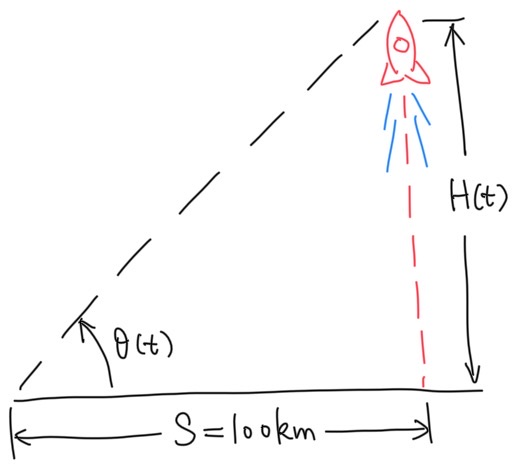
\includegraphics[width=5cm]{./images/ch2/Rocket.jpg}
\end{center}
火箭的高度$H(t)=S\tan\theta(t)$,由此可知
$$H'(t)=S\sec^2\theta(t)\theta'(t),$$
将$S=100$,$\theta(t)=\df{\pi}4$,$\theta'(t)=0.1$带入记得
指定时刻火箭上升的速率为$20$km/s。\hfill$\Box$

\bigskip

3.长度为$6$米的梯子靠在墙角,梯子底部距离墙角$5$米,某一时刻梯子底部开始
向远离墙角的方向滑动,滑动的速度为$0.2$米每秒,问
\begin{enumerate}[(1)]
  \setlength{\itemindent}{1cm}
  \item 此时梯子顶部下滑的速度是多少?
  \item 由梯子、墙面和地面构成的三角形的面积随时间的变化率是多少?
  \item 梯子和地面的夹角的以怎样的速率变化?
\end{enumerate}

[解]:如图,
\begin{center}
	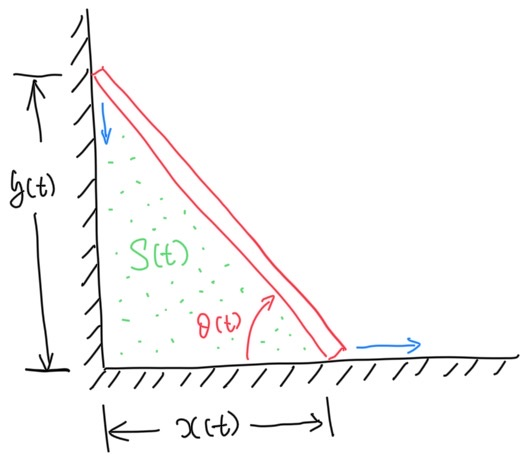
\includegraphics[width=5cm]{./images/ch2/ladder.jpg}
\end{center}
(1)显然$x^2(t)+y^2(t)=36$,两边求导可得
$$x'(t)x(t)+y'(t)y(t)=0\quad
\Rightarrow y'(t)=-\df{x'(t)x(t)}{y(t)},$$
带入$x(t)=5,x'(t)=0.2,y(t)=\sqrt{11}$,可得指定时刻
梯子顶部的下滑速度为$-\df1{\sqrt{11}}$m/s;

(2)$S(t)=\df12x(t)y(t)$,故
$$S'(t)=\df12[x'(t)y(t)+x(t)y'(t)],$$
带入$x(t)=5,x'(t)=0.2,y(t)=\sqrt{11},y'(t)=-\df1{\sqrt{11}}$,
可得所求三角形面积的变化速率为$-\df{7}{5\sqrt{11}}$m$^2$/s;

(3)$\theta(t)=\arctan\df{y(t)}{x(t)}$,故
$$\theta'(t)=\df1{1+\frac{y^2(t)}{x^2(t)}}
\df{y'(t)x(t)-y(t)x'(t)}{x^2(t)}=\df{y'(t)x(t)-y(t)x'(t)}{x^2(t)+y^2(t)},$$
带入$x(t)=5,x'(t)=0.2,y(t)=\sqrt{11},y'(t)=-\df1{\sqrt{11}}$,
可得指定时刻梯子和地面夹角的变化率为$-\df1{5\sqrt{11}}$弧度/s。\hfill$\Box$

\bigskip

4.半径为$a$的圆球渐渐沉入盛有水的半径为$b(b>a)$的圆柱形容器中,若
球的下降速度恒为$c$,求球浸没入水中恰好一半时,容器内水面上升的速率。
(提示:球冠的体积$V=\df{\pi}3(3R-H)H^2$,其中$H$为球冠的高度)

[解]:设$t$时刻,没入水中的球冠高度为$h(t)$,则此时没入水中的球冠体积
$$V(t)=\df{\pi}3(3a-h(t))h^2(t),$$
从而没入水中的球冠体积变换率
$$V'(t)=\pi(2ah(t)-h^2(t))h'(t),$$
相应地,桶内水面升高的速率为
$$H'(t)=\df{V'(t)}{\pi b^2}=\df{2ah(t)-h^2(t)}{b^2}h'(t),$$
带入$h(t)=a,h'(t)=c$,即得所求时刻水面上升的速率为$\df{a^2}{b^2}c$。
\hfill$\Box$

\begin{center}
	\bf 2.6 微分
\end{center}

\bigskip

1.设$y=x^3-2x$,
\begin{enumerate}[(1)]
  \setlength{\itemindent}{1cm}
  \item 计算在$x=2$处当$\Delta x$分别为$1,\;0.1,\;
  0.01$时的$\Delta y$和$\d y$;
  \item 写出$x=2$时$y$的微分表达式。
\end{enumerate}

[解]:
\begin{align*}
	\Delta y&=[(x+\Delta x)^3-2(x+\Delta x)]-(x^3-2x)
	=(3x^2-2)\Delta x+3x\Delta x^2+\Delta x^3,\\
	\d y&=(3x^2-2)\d x=(3x^2-2)\Delta x.
\end{align*}
当$x=2$时,
\begin{align*}
	\Delta y|_{x=2}&
	=10\Delta x+6\Delta x^2+\Delta x^3,\\
	\d y|_{x=2}&=10\Delta x.
\end{align*}
进而
\begin{enumerate}[(i)]
  \item 当$x=2,\Delta x=1$时,$\Delta y=17,\;\d y=10$;
  \item 当$x=2,\Delta x=0.1$时,$\Delta y=1.061,\;\d y=1$;
  \item 当$x=2,\Delta x=0.01$时,$\Delta y=0.1006001,\;\d y=0.1$。
\end{enumerate}
\hfill$\Box$

\bigskip

2.已知$2^{xy}=x-y$,求$\d y|_{x=0}$。

[解]:已知方程两边求微分,可得
$$2^{xy}\ln2(x\d y+y\d x)=\d x-\d y,$$
进而
$$\d y=\df{1-y2^{xy}\ln2}{1+x2^{xy}\ln2}\d x.$$
带入$x=0$即得
$$\d y|_{x=0}=1-y\ln2.$$
\hfill$\Box$

\bigskip

3.设$f(x)=\lim\limits_{t\to\infty}t^2
\left[e^{x+\frac2t}-e^x\right]\sin\df xt$,求$\d f(x)$。

[解]:
\begin{align*}
	f(x)&=\lim\limits_{t\to\infty}t^2
	\left[e^{x+\frac2t}-e^x\right]\sin\df xt
	=e^x\lim\limits_{t\to\infty}t^2
	\left(e^{\frac2t}-1\right)\df xt\\
	&=e^x\lim\limits_{t\to\infty}t^2\df2t\df xt
	=2xe^x.
\end{align*}
故
$$\d f(x)=(2xe^x)'\d x=2e^x(1+x)\d x.$$
\hfill$\Box$

\bigskip

4.略。

5.已知当$h\to 0$时,
$$f(x+2h)-f(x)=h\sqrt{x^2+2x}+\circ(h),$$
求$\d\left[f\left(\df1x\right)\right]$。

[解]:由已知
$$\lim\limits_{h\to0}\df{f(x+2h)-f(x)}{2h}
=\lim\limits_{h\to0}\df{h\sqrt{x^2+2x}+\circ(h)}{2h}
=\df{\sqrt{x^2+2x}}2.
$$
也即$f'(x)=\df{\sqrt{x^2+2x}}2$,故
$$\d\left[f\left(\df1x\right)\right]
=f'\left(\df1x\right)\left(-\df1{x^2}\right)\d x
=-\df{\sqrt{1+2x}}{2x^3}\d x.$$
\hfill$\Box$

\bigskip

6.设$a>0$,$|x|<<a$(表示$|x|$远远小于$a$),证明近似公式
$$\sqrt[n]{a^n+x}\approx a+\df{x}{na^{n-1}}.$$

[解]:记$f(x)=\sqrt[n]{a^n+x}$,显然$f(0)=a$,
又
$$f'(x)=\df1n(a^n+x)^{\frac1n-1}\quad
\Rightarrow f'(0)=\df1{na^{n-1}}.
$$
故由微分的几何意义,当$|x|<<a$时,总有
$$\sqrt[n]{a^n+x}\approx f(0)+f'(0)x
=a+\df{x}{na^{n-1}}.$$
\hfill$\Box$